% Options for packages loaded elsewhere
\PassOptionsToPackage{unicode}{hyperref}
\PassOptionsToPackage{hyphens}{url}
\PassOptionsToPackage{dvipsnames,svgnames,x11names}{xcolor}
%
\documentclass[
  a4paper,
  DIV=11,
  numbers=noendperiod,
  oneside,
  open=any]{scrreprt}

\usepackage{amsmath,amssymb}
\usepackage{setspace}
\usepackage{iftex}
\ifPDFTeX
  \usepackage[T1]{fontenc}
  \usepackage[utf8]{inputenc}
  \usepackage{textcomp} % provide euro and other symbols
\else % if luatex or xetex
  \usepackage{unicode-math}
  \defaultfontfeatures{Scale=MatchLowercase}
  \defaultfontfeatures[\rmfamily]{Ligatures=TeX,Scale=1}
\fi
\usepackage{lmodern}
\ifPDFTeX\else  
    % xetex/luatex font selection
    \setmainfont[]{Times New Roman}
    \setsansfont[]{Arial}
    \setmonofont[]{Courier New}
\fi
% Use upquote if available, for straight quotes in verbatim environments
\IfFileExists{upquote.sty}{\usepackage{upquote}}{}
\IfFileExists{microtype.sty}{% use microtype if available
  \usepackage[]{microtype}
  \UseMicrotypeSet[protrusion]{basicmath} % disable protrusion for tt fonts
}{}
\makeatletter
\@ifundefined{KOMAClassName}{% if non-KOMA class
  \IfFileExists{parskip.sty}{%
    \usepackage{parskip}
  }{% else
    \setlength{\parindent}{0pt}
    \setlength{\parskip}{6pt plus 2pt minus 1pt}}
}{% if KOMA class
  \KOMAoptions{parskip=half}}
\makeatother
\usepackage{xcolor}
\usepackage[a4paper,left=2cm,right=2cm,top=2.5cm,bottom=2.5cm,columnsep=0cm]{geometry}
\setlength{\emergencystretch}{3em} % prevent overfull lines
\setcounter{secnumdepth}{2}
% Make \paragraph and \subparagraph free-standing
\makeatletter
\ifx\paragraph\undefined\else
  \let\oldparagraph\paragraph
  \renewcommand{\paragraph}{
    \@ifstar
      \xxxParagraphStar
      \xxxParagraphNoStar
  }
  \newcommand{\xxxParagraphStar}[1]{\oldparagraph*{#1}\mbox{}}
  \newcommand{\xxxParagraphNoStar}[1]{\oldparagraph{#1}\mbox{}}
\fi
\ifx\subparagraph\undefined\else
  \let\oldsubparagraph\subparagraph
  \renewcommand{\subparagraph}{
    \@ifstar
      \xxxSubParagraphStar
      \xxxSubParagraphNoStar
  }
  \newcommand{\xxxSubParagraphStar}[1]{\oldsubparagraph*{#1}\mbox{}}
  \newcommand{\xxxSubParagraphNoStar}[1]{\oldsubparagraph{#1}\mbox{}}
\fi
\makeatother

\usepackage{color}
\usepackage{fancyvrb}
\newcommand{\VerbBar}{|}
\newcommand{\VERB}{\Verb[commandchars=\\\{\}]}
\DefineVerbatimEnvironment{Highlighting}{Verbatim}{commandchars=\\\{\}}
% Add ',fontsize=\small' for more characters per line
\usepackage{framed}
\definecolor{shadecolor}{RGB}{241,243,245}
\newenvironment{Shaded}{\begin{snugshade}}{\end{snugshade}}
\newcommand{\AlertTok}[1]{\textcolor[rgb]{0.68,0.00,0.00}{#1}}
\newcommand{\AnnotationTok}[1]{\textcolor[rgb]{0.37,0.37,0.37}{#1}}
\newcommand{\AttributeTok}[1]{\textcolor[rgb]{0.40,0.45,0.13}{#1}}
\newcommand{\BaseNTok}[1]{\textcolor[rgb]{0.68,0.00,0.00}{#1}}
\newcommand{\BuiltInTok}[1]{\textcolor[rgb]{0.00,0.23,0.31}{#1}}
\newcommand{\CharTok}[1]{\textcolor[rgb]{0.13,0.47,0.30}{#1}}
\newcommand{\CommentTok}[1]{\textcolor[rgb]{0.37,0.37,0.37}{#1}}
\newcommand{\CommentVarTok}[1]{\textcolor[rgb]{0.37,0.37,0.37}{\textit{#1}}}
\newcommand{\ConstantTok}[1]{\textcolor[rgb]{0.56,0.35,0.01}{#1}}
\newcommand{\ControlFlowTok}[1]{\textcolor[rgb]{0.00,0.23,0.31}{\textbf{#1}}}
\newcommand{\DataTypeTok}[1]{\textcolor[rgb]{0.68,0.00,0.00}{#1}}
\newcommand{\DecValTok}[1]{\textcolor[rgb]{0.68,0.00,0.00}{#1}}
\newcommand{\DocumentationTok}[1]{\textcolor[rgb]{0.37,0.37,0.37}{\textit{#1}}}
\newcommand{\ErrorTok}[1]{\textcolor[rgb]{0.68,0.00,0.00}{#1}}
\newcommand{\ExtensionTok}[1]{\textcolor[rgb]{0.00,0.23,0.31}{#1}}
\newcommand{\FloatTok}[1]{\textcolor[rgb]{0.68,0.00,0.00}{#1}}
\newcommand{\FunctionTok}[1]{\textcolor[rgb]{0.28,0.35,0.67}{#1}}
\newcommand{\ImportTok}[1]{\textcolor[rgb]{0.00,0.46,0.62}{#1}}
\newcommand{\InformationTok}[1]{\textcolor[rgb]{0.37,0.37,0.37}{#1}}
\newcommand{\KeywordTok}[1]{\textcolor[rgb]{0.00,0.23,0.31}{\textbf{#1}}}
\newcommand{\NormalTok}[1]{\textcolor[rgb]{0.00,0.23,0.31}{#1}}
\newcommand{\OperatorTok}[1]{\textcolor[rgb]{0.37,0.37,0.37}{#1}}
\newcommand{\OtherTok}[1]{\textcolor[rgb]{0.00,0.23,0.31}{#1}}
\newcommand{\PreprocessorTok}[1]{\textcolor[rgb]{0.68,0.00,0.00}{#1}}
\newcommand{\RegionMarkerTok}[1]{\textcolor[rgb]{0.00,0.23,0.31}{#1}}
\newcommand{\SpecialCharTok}[1]{\textcolor[rgb]{0.37,0.37,0.37}{#1}}
\newcommand{\SpecialStringTok}[1]{\textcolor[rgb]{0.13,0.47,0.30}{#1}}
\newcommand{\StringTok}[1]{\textcolor[rgb]{0.13,0.47,0.30}{#1}}
\newcommand{\VariableTok}[1]{\textcolor[rgb]{0.07,0.07,0.07}{#1}}
\newcommand{\VerbatimStringTok}[1]{\textcolor[rgb]{0.13,0.47,0.30}{#1}}
\newcommand{\WarningTok}[1]{\textcolor[rgb]{0.37,0.37,0.37}{\textit{#1}}}

\providecommand{\tightlist}{%
  \setlength{\itemsep}{0pt}\setlength{\parskip}{0pt}}\usepackage{longtable,booktabs,array}
\usepackage{calc} % for calculating minipage widths
% Correct order of tables after \paragraph or \subparagraph
\usepackage{etoolbox}
\makeatletter
\patchcmd\longtable{\par}{\if@noskipsec\mbox{}\fi\par}{}{}
\makeatother
% Allow footnotes in longtable head/foot
\IfFileExists{footnotehyper.sty}{\usepackage{footnotehyper}}{\usepackage{footnote}}
\makesavenoteenv{longtable}
\usepackage{graphicx}
\makeatletter
\def\maxwidth{\ifdim\Gin@nat@width>\linewidth\linewidth\else\Gin@nat@width\fi}
\def\maxheight{\ifdim\Gin@nat@height>\textheight\textheight\else\Gin@nat@height\fi}
\makeatother
% Scale images if necessary, so that they will not overflow the page
% margins by default, and it is still possible to overwrite the defaults
% using explicit options in \includegraphics[width, height, ...]{}
\setkeys{Gin}{width=\maxwidth,height=\maxheight,keepaspectratio}
% Set default figure placement to htbp
\makeatletter
\def\fps@figure{htbp}
\makeatother
% definitions for citeproc citations
\NewDocumentCommand\citeproctext{}{}
\NewDocumentCommand\citeproc{mm}{%
  \begingroup\def\citeproctext{#2}\cite{#1}\endgroup}
\makeatletter
 % allow citations to break across lines
 \let\@cite@ofmt\@firstofone
 % avoid brackets around text for \cite:
 \def\@biblabel#1{}
 \def\@cite#1#2{{#1\if@tempswa , #2\fi}}
\makeatother
\newlength{\cslhangindent}
\setlength{\cslhangindent}{1.5em}
\newlength{\csllabelwidth}
\setlength{\csllabelwidth}{3em}
\newenvironment{CSLReferences}[2] % #1 hanging-indent, #2 entry-spacing
 {\begin{list}{}{%
  \setlength{\itemindent}{0pt}
  \setlength{\leftmargin}{0pt}
  \setlength{\parsep}{0pt}
  % turn on hanging indent if param 1 is 1
  \ifodd #1
   \setlength{\leftmargin}{\cslhangindent}
   \setlength{\itemindent}{-1\cslhangindent}
  \fi
  % set entry spacing
  \setlength{\itemsep}{#2\baselineskip}}}
 {\end{list}}
\usepackage{calc}
\newcommand{\CSLBlock}[1]{\hfill\break\parbox[t]{\linewidth}{\strut\ignorespaces#1\strut}}
\newcommand{\CSLLeftMargin}[1]{\parbox[t]{\csllabelwidth}{\strut#1\strut}}
\newcommand{\CSLRightInline}[1]{\parbox[t]{\linewidth - \csllabelwidth}{\strut#1\strut}}
\newcommand{\CSLIndent}[1]{\hspace{\cslhangindent}#1}

\usepackage{fontspec}
\setmainfont{TeX Gyre Termes}[Scale=1.2]
\usepackage{unicode-math}
\KOMAoption{captions}{tableheading}
\makeatletter
\@ifpackageloaded{tcolorbox}{}{\usepackage[skins,breakable]{tcolorbox}}
\@ifpackageloaded{fontawesome5}{}{\usepackage{fontawesome5}}
\definecolor{quarto-callout-color}{HTML}{909090}
\definecolor{quarto-callout-note-color}{HTML}{0758E5}
\definecolor{quarto-callout-important-color}{HTML}{CC1914}
\definecolor{quarto-callout-warning-color}{HTML}{EB9113}
\definecolor{quarto-callout-tip-color}{HTML}{00A047}
\definecolor{quarto-callout-caution-color}{HTML}{FC5300}
\definecolor{quarto-callout-color-frame}{HTML}{acacac}
\definecolor{quarto-callout-note-color-frame}{HTML}{4582ec}
\definecolor{quarto-callout-important-color-frame}{HTML}{d9534f}
\definecolor{quarto-callout-warning-color-frame}{HTML}{f0ad4e}
\definecolor{quarto-callout-tip-color-frame}{HTML}{02b875}
\definecolor{quarto-callout-caution-color-frame}{HTML}{fd7e14}
\makeatother
\makeatletter
\@ifpackageloaded{bookmark}{}{\usepackage{bookmark}}
\makeatother
\makeatletter
\@ifpackageloaded{caption}{}{\usepackage{caption}}
\AtBeginDocument{%
\ifdefined\contentsname
  \renewcommand*\contentsname{Table of contents}
\else
  \newcommand\contentsname{Table of contents}
\fi
\ifdefined\listfigurename
  \renewcommand*\listfigurename{List of Figures}
\else
  \newcommand\listfigurename{List of Figures}
\fi
\ifdefined\listtablename
  \renewcommand*\listtablename{List of Tables}
\else
  \newcommand\listtablename{List of Tables}
\fi
\ifdefined\figurename
  \renewcommand*\figurename{Figure}
\else
  \newcommand\figurename{Figure}
\fi
\ifdefined\tablename
  \renewcommand*\tablename{Table}
\else
  \newcommand\tablename{Table}
\fi
}
\@ifpackageloaded{float}{}{\usepackage{float}}
\floatstyle{ruled}
\@ifundefined{c@chapter}{\newfloat{codelisting}{h}{lop}}{\newfloat{codelisting}{h}{lop}[chapter]}
\floatname{codelisting}{Listing}
\newcommand*\listoflistings{\listof{codelisting}{List of Listings}}
\makeatother
\makeatletter
\makeatother
\makeatletter
\@ifpackageloaded{caption}{}{\usepackage{caption}}
\@ifpackageloaded{subcaption}{}{\usepackage{subcaption}}
\makeatother
\makeatletter
\@ifpackageloaded{sidenotes}{}{\usepackage{sidenotes}}
\@ifpackageloaded{marginnote}{}{\usepackage{marginnote}}
\makeatother

\ifLuaTeX
  \usepackage{selnolig}  % disable illegal ligatures
\fi
\usepackage{bookmark}

\IfFileExists{xurl.sty}{\usepackage{xurl}}{} % add URL line breaks if available
\urlstyle{same} % disable monospaced font for URLs
\hypersetup{
  pdftitle={DSP\_DNS\_Book},
  pdfauthor={Michał Lesiowski},
  colorlinks=true,
  linkcolor={blue},
  filecolor={Maroon},
  citecolor={Blue},
  urlcolor={Blue},
  pdfcreator={LaTeX via pandoc}}


\title{DSP\_DNS\_Book}
\author{Michał Lesiowski}
\date{2024-09-23}

\begin{document}
\maketitle

\renewcommand*\contentsname{Table of contents}
{
\hypersetup{linkcolor=}
\setcounter{tocdepth}{2}
\tableofcontents
}

\setstretch{1.25}
\bookmarksetup{startatroot}

\chapter*{Preface}\label{preface}
\addcontentsline{toc}{chapter}{Preface}

\markboth{Preface}{Preface}

This is a Quarto book.

To learn more about Quarto books visit
\url{https://quarto.org/docs/books}.

\begin{Shaded}
\begin{Highlighting}[]
\DecValTok{1} \SpecialCharTok{+} \DecValTok{1}
\end{Highlighting}
\end{Shaded}

\begin{verbatim}
[1] 2
\end{verbatim}

\begin{Shaded}
\begin{Highlighting}[]
\DecValTok{13} \SpecialCharTok{/} \DecValTok{3}
\end{Highlighting}
\end{Shaded}

\begin{verbatim}
[1] 4.333333
\end{verbatim}

Test test 123 i inny test

\bookmarksetup{startatroot}

\chapter*{Wprowadzenie}\label{wprowadzenie}
\addcontentsline{toc}{chapter}{Wprowadzenie}

\markboth{Wprowadzenie}{Wprowadzenie}

\section*{Cel dokumentu}\label{cel-dokumentu}
\addcontentsline{toc}{section}{Cel dokumentu}

\markright{Cel dokumentu}

\section*{Zakres systemu}\label{zakres-systemu}
\addcontentsline{toc}{section}{Zakres systemu}

\markright{Zakres systemu}

\section*{Definicje, akronimy,
skróty}\label{definicje-akronimy-skruxf3ty}
\addcontentsline{toc}{section}{Definicje, akronimy, skróty}

\markright{Definicje, akronimy, skróty}

\section*{Dokumenty referencyjne}\label{dokumenty-referencyjne}
\addcontentsline{toc}{section}{Dokumenty referencyjne}

\markright{Dokumenty referencyjne}

\section*{Odbiorcy dokumentu}\label{odbiorcy-dokumentu}
\addcontentsline{toc}{section}{Odbiorcy dokumentu}

\markright{Odbiorcy dokumentu}

\marginnote{\begin{footnotesize}

\begin{tcolorbox}[enhanced jigsaw, bottomrule=.15mm, titlerule=0mm, colbacktitle=quarto-callout-note-color!10!white, coltitle=black, rightrule=.15mm, opacitybacktitle=0.6, colframe=quarto-callout-note-color-frame, colback=white, breakable, arc=.35mm, toptitle=1mm, leftrule=.75mm, bottomtitle=1mm, title=\textcolor{quarto-callout-note-color}{\faInfo}\hspace{0.5em}{Uwaga}, toprule=.15mm, left=2mm, opacityback=0]

To jest przykładowy callout w sekcji bocznej.

\end{tcolorbox}

\end{footnotesize}}

\begin{figure}

\begin{minipage}{0.33\linewidth}
This is a template for a simple Quarto book output to html, PDF or docx
format. It includes a GitHub Action that will build the website
automatically when you make changes to the files. The NOAA palette and
fonts has been added to theme.scss. The webpage will be on the gh-pages
branch. Serving the website files from this branch is a common way to
keep all the website files from cluttering your main
branch\end{minipage}%
%
\begin{minipage}{0.33\linewidth}
This is a template for a simple Quarto book output to html, PDF or docx
format. It includes a GitHub Action that will build the website
automatically when you make changes to the files. The NOAA palette and
fonts has been added to theme.scss. The webpage will be on the gh-pages
branch. Serving the website files from this branch is a common way to
keep all the website files from cluttering your main
branch\end{minipage}%
%
\begin{minipage}{0.33\linewidth}
This is a template for a simple Quarto book output to html, PDF or docx
format. It includes a GitHub Action that will build the website
automatically when you make changes to the files. The NOAA palette and
fonts has been added to theme.scss. The webpage will be on the gh-pages
branch. Serving the website files from this branch is a common way to
keep all the website files from cluttering your main
branch\end{minipage}%

\end{figure}%

\begin{center}\rule{0.5\linewidth}{0.5pt}\end{center}

This is a template for a simple Quarto book output to html, PDF or docx
format. It includes a GitHub Action that will build the website
automatically when you make changes to the files.

This is a template for a simple Quarto book output to html, PDF or docx
format. It includes a GitHub Action that will build the website
automatically when you make changes to the files.

\begin{longtable}[]{@{}ll@{}}
\caption{Fruit prices}\tabularnewline
\toprule\noalign{}
fruit & price \\
\midrule\noalign{}
\endfirsthead
\toprule\noalign{}
fruit & price \\
\midrule\noalign{}
\endhead
\bottomrule\noalign{}
\endlastfoot
apple & 2.05 \\
pear & 1.37 \\
orange & 3.09 \\
\end{longtable}

\subsection*{Grid tables}\label{grid-tables}
\addcontentsline{toc}{subsection}{Grid tables}

Bardziej zaawansowany typ np dodatkowe paragrafy, bloki kodu, listy

\begin{longtable}[]{@{}
  >{\raggedright\arraybackslash}p{(\columnwidth - 4\tabcolsep) * \real{0.1667}}
  >{\raggedright\arraybackslash}p{(\columnwidth - 4\tabcolsep) * \real{0.1667}}
  >{\raggedright\arraybackslash}p{(\columnwidth - 4\tabcolsep) * \real{0.2917}}@{}}
\toprule\noalign{}
\begin{minipage}[b]{\linewidth}\raggedright
Fruit
\end{minipage} & \begin{minipage}[b]{\linewidth}\raggedright
Price
\end{minipage} & \begin{minipage}[b]{\linewidth}\raggedright
Advantages
\end{minipage} \\
\midrule\noalign{}
\endhead
\bottomrule\noalign{}
\endlastfoot
Bananas & \$1.34 & \begin{minipage}[t]{\linewidth}\raggedright
\begin{itemize}
\tightlist
\item
  built-in wrapper
\item
  bright color
\end{itemize}
\end{minipage} \\
Oranges & \$2.10 & \begin{minipage}[t]{\linewidth}\raggedright
\begin{itemize}
\tightlist
\item
  cures scurvy
\item
  tasty
\end{itemize}
\end{minipage} \\
\end{longtable}

\section*{Link do 2 pages}\label{link-do-2-pages}
\addcontentsline{toc}{section}{Link do 2 pages}

\markright{Link do 2 pages}

\hyperref[podziaux5cux25C5ux5cux2582-na-dwie-kolumny]{intro}

\section*{Funckje jakie oczekuje od końcowego
rozwiązania:}\label{funckje-jakie-oczekuje-od-koux144cowego-rozwiux105zania}
\addcontentsline{toc}{section}{Funckje jakie oczekuje od końcowego
rozwiązania:}

\markright{Funckje jakie oczekuje od końcowego rozwiązania:}

\begin{itemize}
\item
  Output do: PDF, DOCX, HTML
\item
  Github Actions that will build website automatically when I make
  changes to the files
\item
  Obsługa diagramów
\item
  Konfigruacja pełna layoutu np. wygląd, czcionki poprzez theme.csss
\item
  Templates dla
\end{itemize}

\bookmarksetup{startatroot}

\chapter{Introduction}\label{introduction}

This is a book created from markdown and executable code.

See Knuth (1984) for additional discussion of literate programming.

\begin{Shaded}
\begin{Highlighting}[]
\DecValTok{1} \SpecialCharTok{+} \DecValTok{1}
\end{Highlighting}
\end{Shaded}

\begin{verbatim}
[1] 2
\end{verbatim}

\section{Interactivity Test}\label{interactivity-test}

\section{Test cross reference}\label{test-cross-reference}

See Figure~\ref{fig-obraz2} for an illustration

\hyperref[koniec]{Skocz do koniec}

\section{Test list of figures}\label{test-list-of-figures}

\listoffigures

\section{Rozdział kolejny}\label{rozdziaux142-kolejny}

Test

\begin{longtable}[]{@{}lll@{}}
\toprule\noalign{}
Col1 & Col2 & Col3 \\
\midrule\noalign{}
\endhead
\bottomrule\noalign{}
\endlastfoot
1 & 2 & 3 \\
1 & 2 & 3 \\
3 & 3 & 3 \\
\end{longtable}

\section{Test sekcji}\label{test-sekcji}

Poniżej RAW content z HTML

\section{Rozdział drugi}\label{rozdziaux142-drugi}

Drugi rozdział

\subsection{Trzeci podrozdział}\label{trzeci-podrozdziaux142}

Trzeci itd.. You can also do this on a per-format basis (if for example
you want to provide a higher resolution image for EPUB and a lower
resolution image for HTML to reduce download time). For example:

{\marginnote{\begin{footnotesize}By ``right format'', we mean that the
data is tidy, and ready to be summarised and
graphed.\end{footnotesize}}}

Quarto Pub is a free publishing service for content created with Quarto.
Quarto Pub is ideal for blogs, course or project websites, books,
presentations, and personal hobby sites.

It's important to note that all documents and sites published to Quarto
Pub are publicly visible. You should only publish content you wish to
share publicly.

\begin{tcolorbox}[enhanced jigsaw, bottomrule=.15mm, titlerule=0mm, colbacktitle=quarto-callout-caution-color!10!white, coltitle=black, rightrule=.15mm, opacitybacktitle=0.6, colframe=quarto-callout-caution-color-frame, colback=white, breakable, arc=.35mm, toptitle=1mm, leftrule=.75mm, bottomtitle=1mm, title=\textcolor{quarto-callout-caution-color}{\faFire}\hspace{0.5em}{Caution}, toprule=.15mm, left=2mm, opacityback=0]

Tu znajduje się zwijana sekcja w boxie callout typu caution

\end{tcolorbox}

\begin{tcolorbox}[enhanced jigsaw, bottomrule=.15mm, titlerule=0mm, colbacktitle=quarto-callout-tip-color!10!white, coltitle=black, rightrule=.15mm, opacitybacktitle=0.6, colframe=quarto-callout-tip-color-frame, colback=white, breakable, arc=.35mm, toptitle=1mm, leftrule=.75mm, bottomtitle=1mm, title=\textcolor{quarto-callout-tip-color}{\faLightbulb}\hspace{0.5em}{Tip}, toprule=.15mm, left=2mm, opacityback=0]

Altair is based on Vega-Lite, a high-level grammar of interactive
graphics

\end{tcolorbox}

Właściwe linki i tu przykładowy odnośnik do mojej {[}{[}books{]}{]}
książek

\begin{tcolorbox}[enhanced jigsaw, bottomrule=.15mm, titlerule=0mm, colbacktitle=quarto-callout-note-color!10!white, coltitle=black, rightrule=.15mm, opacitybacktitle=0.6, colframe=quarto-callout-note-color-frame, colback=white, breakable, arc=.35mm, toptitle=1mm, leftrule=.75mm, bottomtitle=1mm, title=\textcolor{quarto-callout-note-color}{\faInfo}\hspace{0.5em}{Note}, toprule=.15mm, left=2mm, opacityback=0]

A tu znajduje się callout note

\end{tcolorbox}

\begin{quote}
Cytacik lub wcięcie takie coś\ldots{}
\end{quote}

If you haven't published to Quarto Pub before, the publish command will
prompt you to authenticate. After confirming that you want to publish,
your content will be rendered and deployed, and then a browser opened to
view your site.

A jeśli chcemy umieścić kod to możemy to zrobić przy użyciu takiej
dyrektywy jak poniżej. Może być ona też zwijana i rozwijana. To się
określa w konigu yaml/

\begin{Shaded}
\begin{Highlighting}[]
\FunctionTok{library}\NormalTok{(tidyverse)}
\NormalTok{penguins }\OtherTok{\textless{}{-}} \FunctionTok{read.csv}\NormalTok{(}\StringTok{\textquotesingle{}https://raw.githubusercontent.com/rfordatascience/tidytuesday/master/data/2020/2020{-}07{-}28/penguins.csv\textquotesingle{}}\NormalTok{)}\SpecialCharTok{\%\textgreater{}\%}
  \FunctionTok{drop\_na}\NormalTok{()}
\FunctionTok{head}\NormalTok{(penguins)}
\end{Highlighting}
\end{Shaded}

\begin{verbatim}
  species    island bill_length_mm bill_depth_mm flipper_length_mm body_mass_g
1  Adelie Torgersen           39.1          18.7               181        3750
2  Adelie Torgersen           39.5          17.4               186        3800
3  Adelie Torgersen           40.3          18.0               195        3250
4  Adelie Torgersen           36.7          19.3               193        3450
5  Adelie Torgersen           39.3          20.6               190        3650
6  Adelie Torgersen           38.9          17.8               181        3625
     sex year
1   male 2007
2 female 2007
3 female 2007
4 female 2007
5   male 2007
6 female 2007
\end{verbatim}

We've removed missing values here, which means that the data has 333
rows now{[}\^{}1{]}. Ten indeks górny przypis \^{}1 coś nie chce
zabanglać

If you have an existing Quarto Pub site that you want to publish to, you
should manually create a \_publish.yml file that looks like the example
above, but with the appropriate id and url values for your site.

\begin{figure}[H]

{\centering 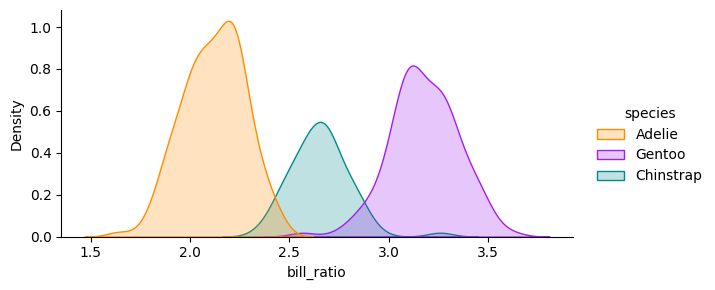
\includegraphics[width=3.125in,height=\textheight]{graph1.png}

}

\caption{Właściwy opis wykresu}

\end{figure}%

\subsection{Podział na dwie kolumny}\label{podziaux142-na-dwie-kolumny}

Poniżej demo jak podzielić przestrzeń na 2 kolumny

\begin{figure}

\begin{minipage}{0.50\linewidth}

\begin{figure}[H]

\centering{

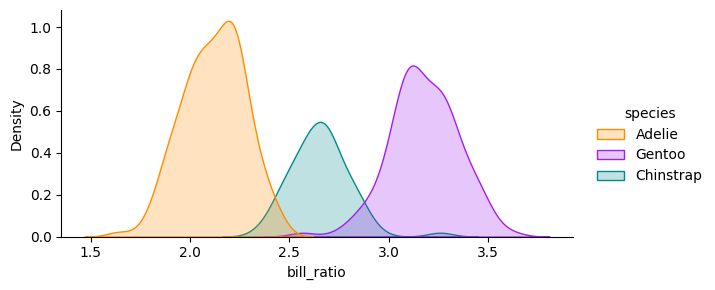
\includegraphics[width=3.125in,height=\textheight]{graph1.png}

}

\caption{\label{fig-obraz1}Właściwy opis wykresu}

\end{figure}%

\end{minipage}%
%
\begin{minipage}{0.50\linewidth}

\begin{figure}[H]

\centering{

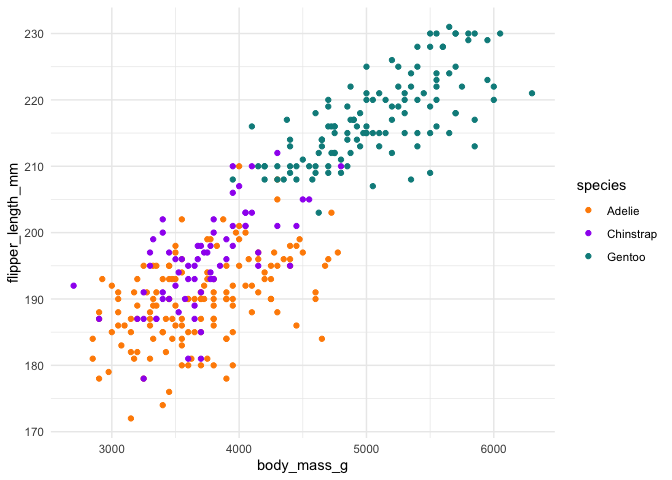
\includegraphics[width=3.125in,height=\textheight]{graph2.png}

}

\caption{\label{fig-obraz2}Właściwy opis wykresu}

\end{figure}%

\end{minipage}%

\end{figure}%

The average bill length is 43.9927928 mm and the average bill depth is
17.1648649 mm.

The data was collected between 2007 and 2009

\subsection{Zewnętrzne źródło}\label{zewnux119trzne-ux17aruxf3dux142o}

\begin{figure}

\centering{

}

\caption{\label{fig-elephant}Elephant}

\end{figure}%

\subsection{Dyrektywa na całą
szerokość}\label{dyrektywa-na-caux142ux105-szerokoux15bux107}

\begin{figure*}

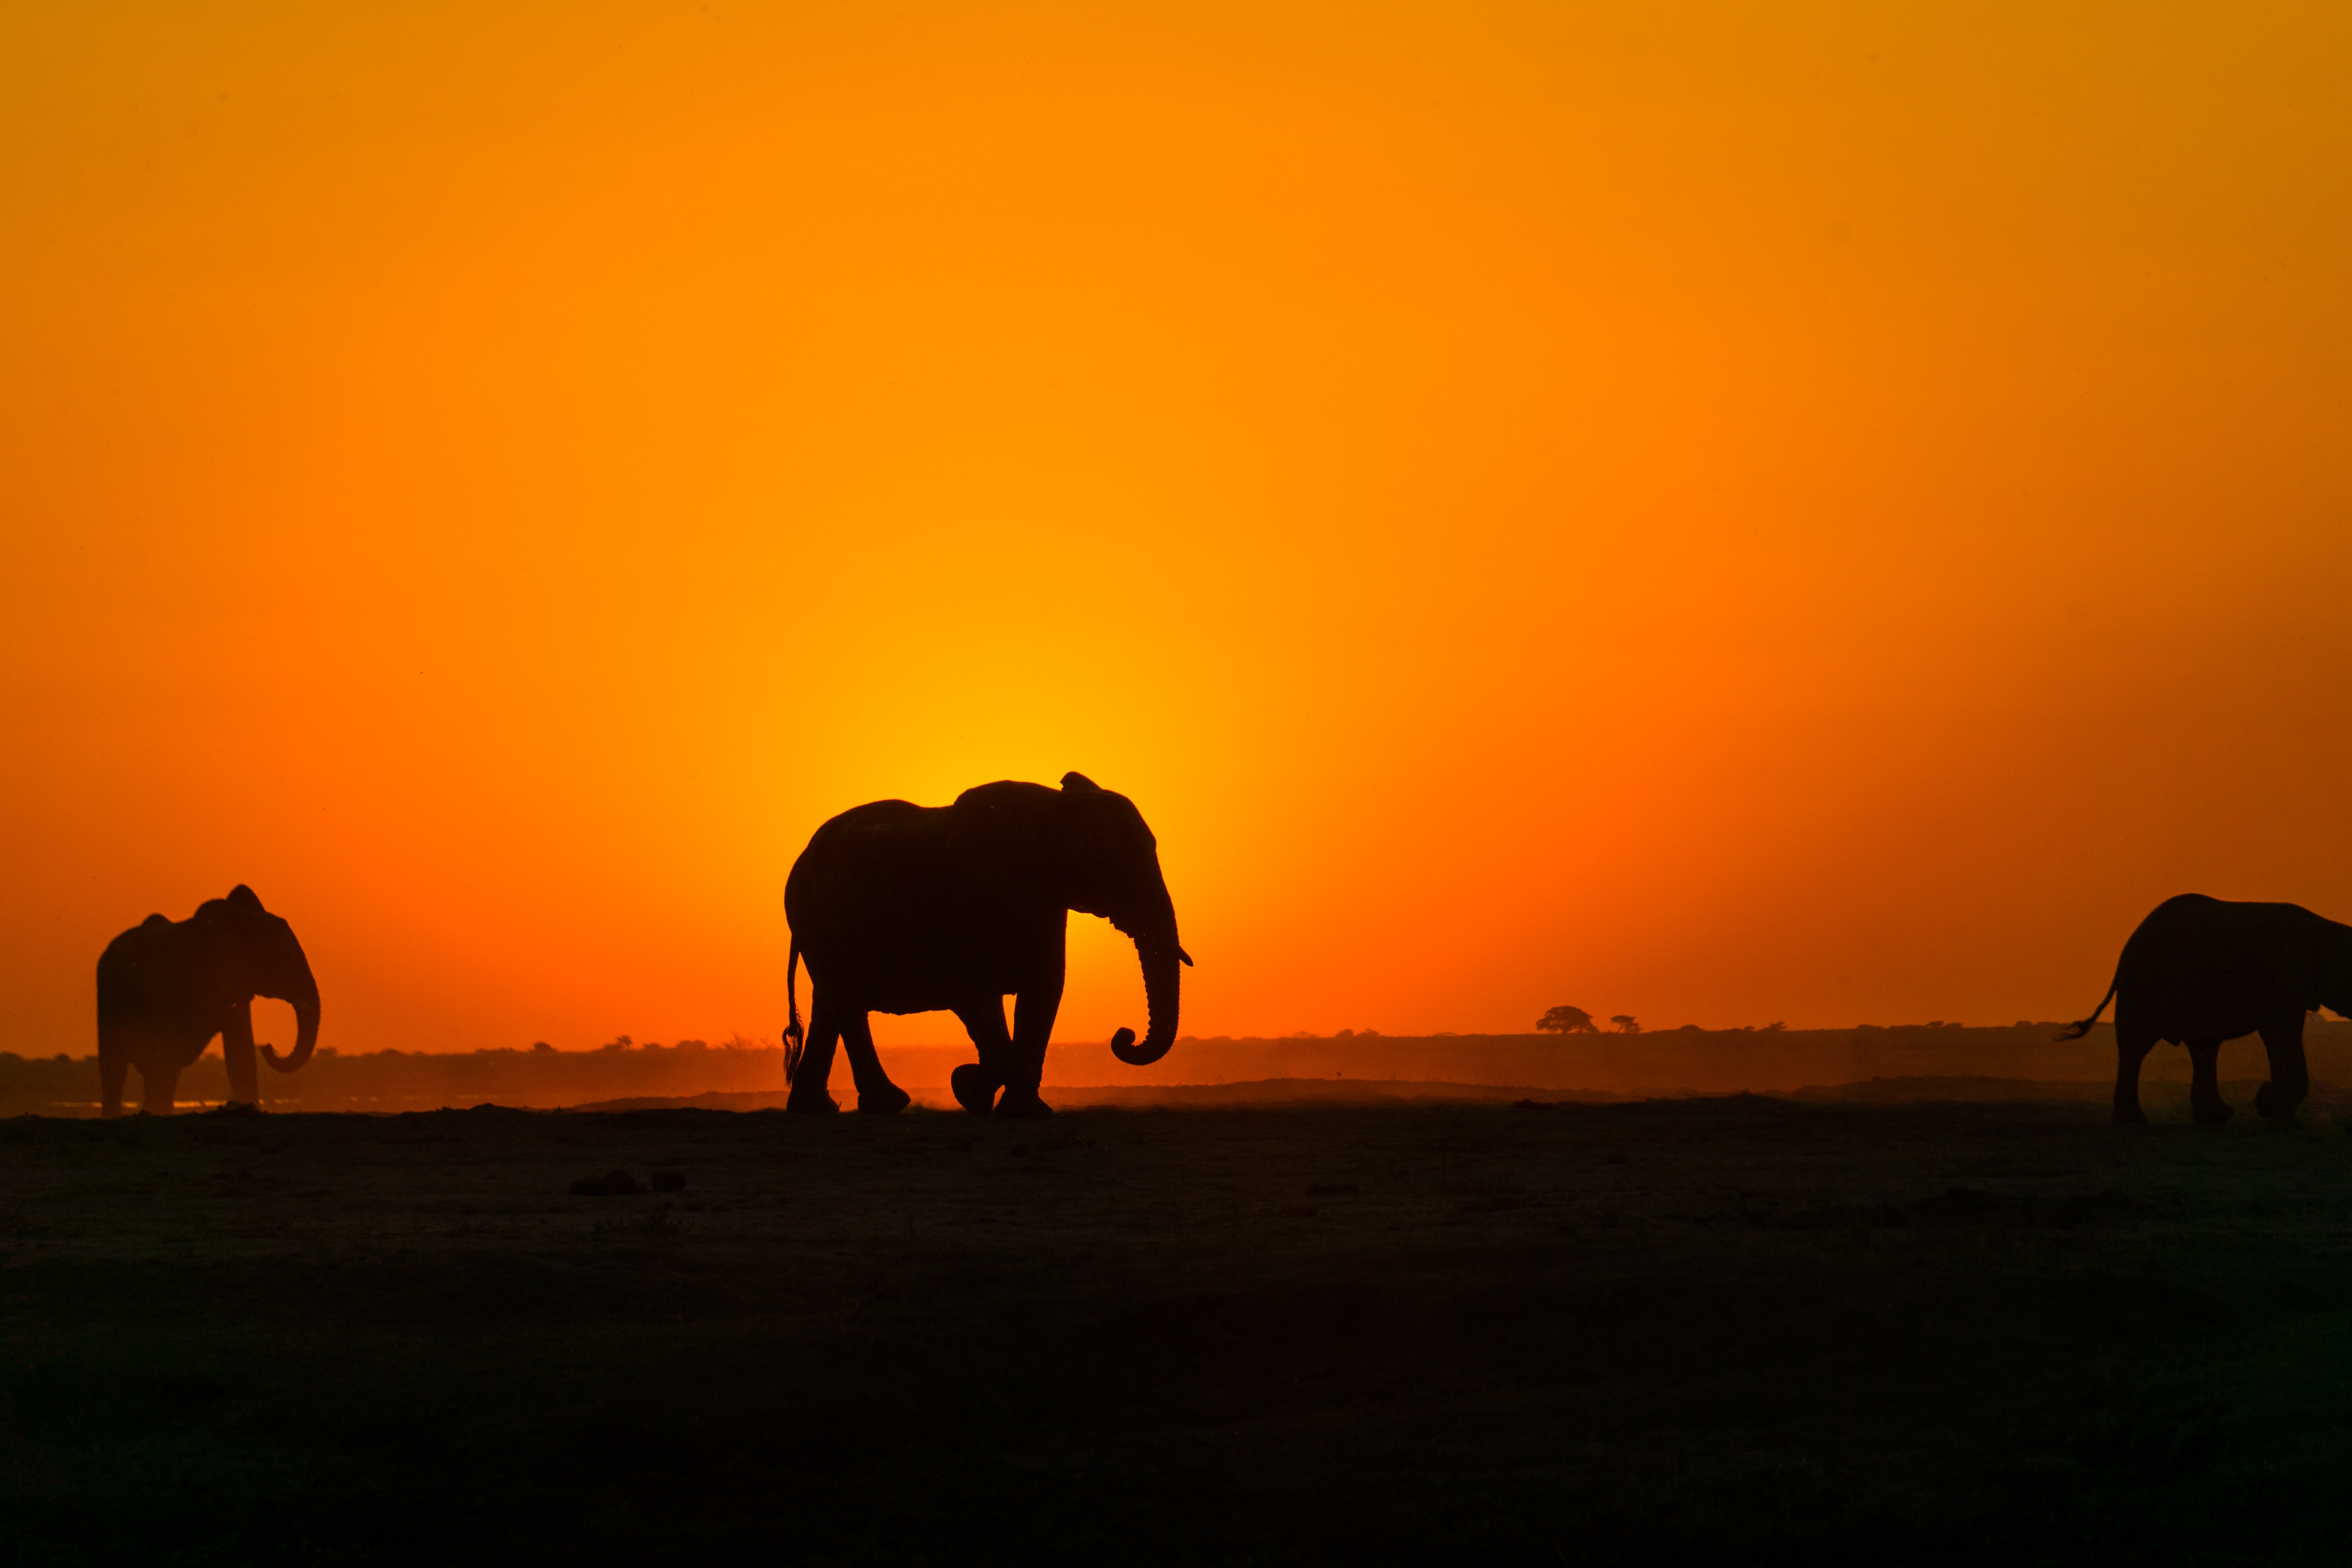
\includegraphics{elephant.jpg}

\end{figure*}%

\subsection{Dyrektywa na całe okno}\label{dyrektywa-na-caux142e-okno}

\begin{figure*}%
\begin{figure}[H]

{\centering 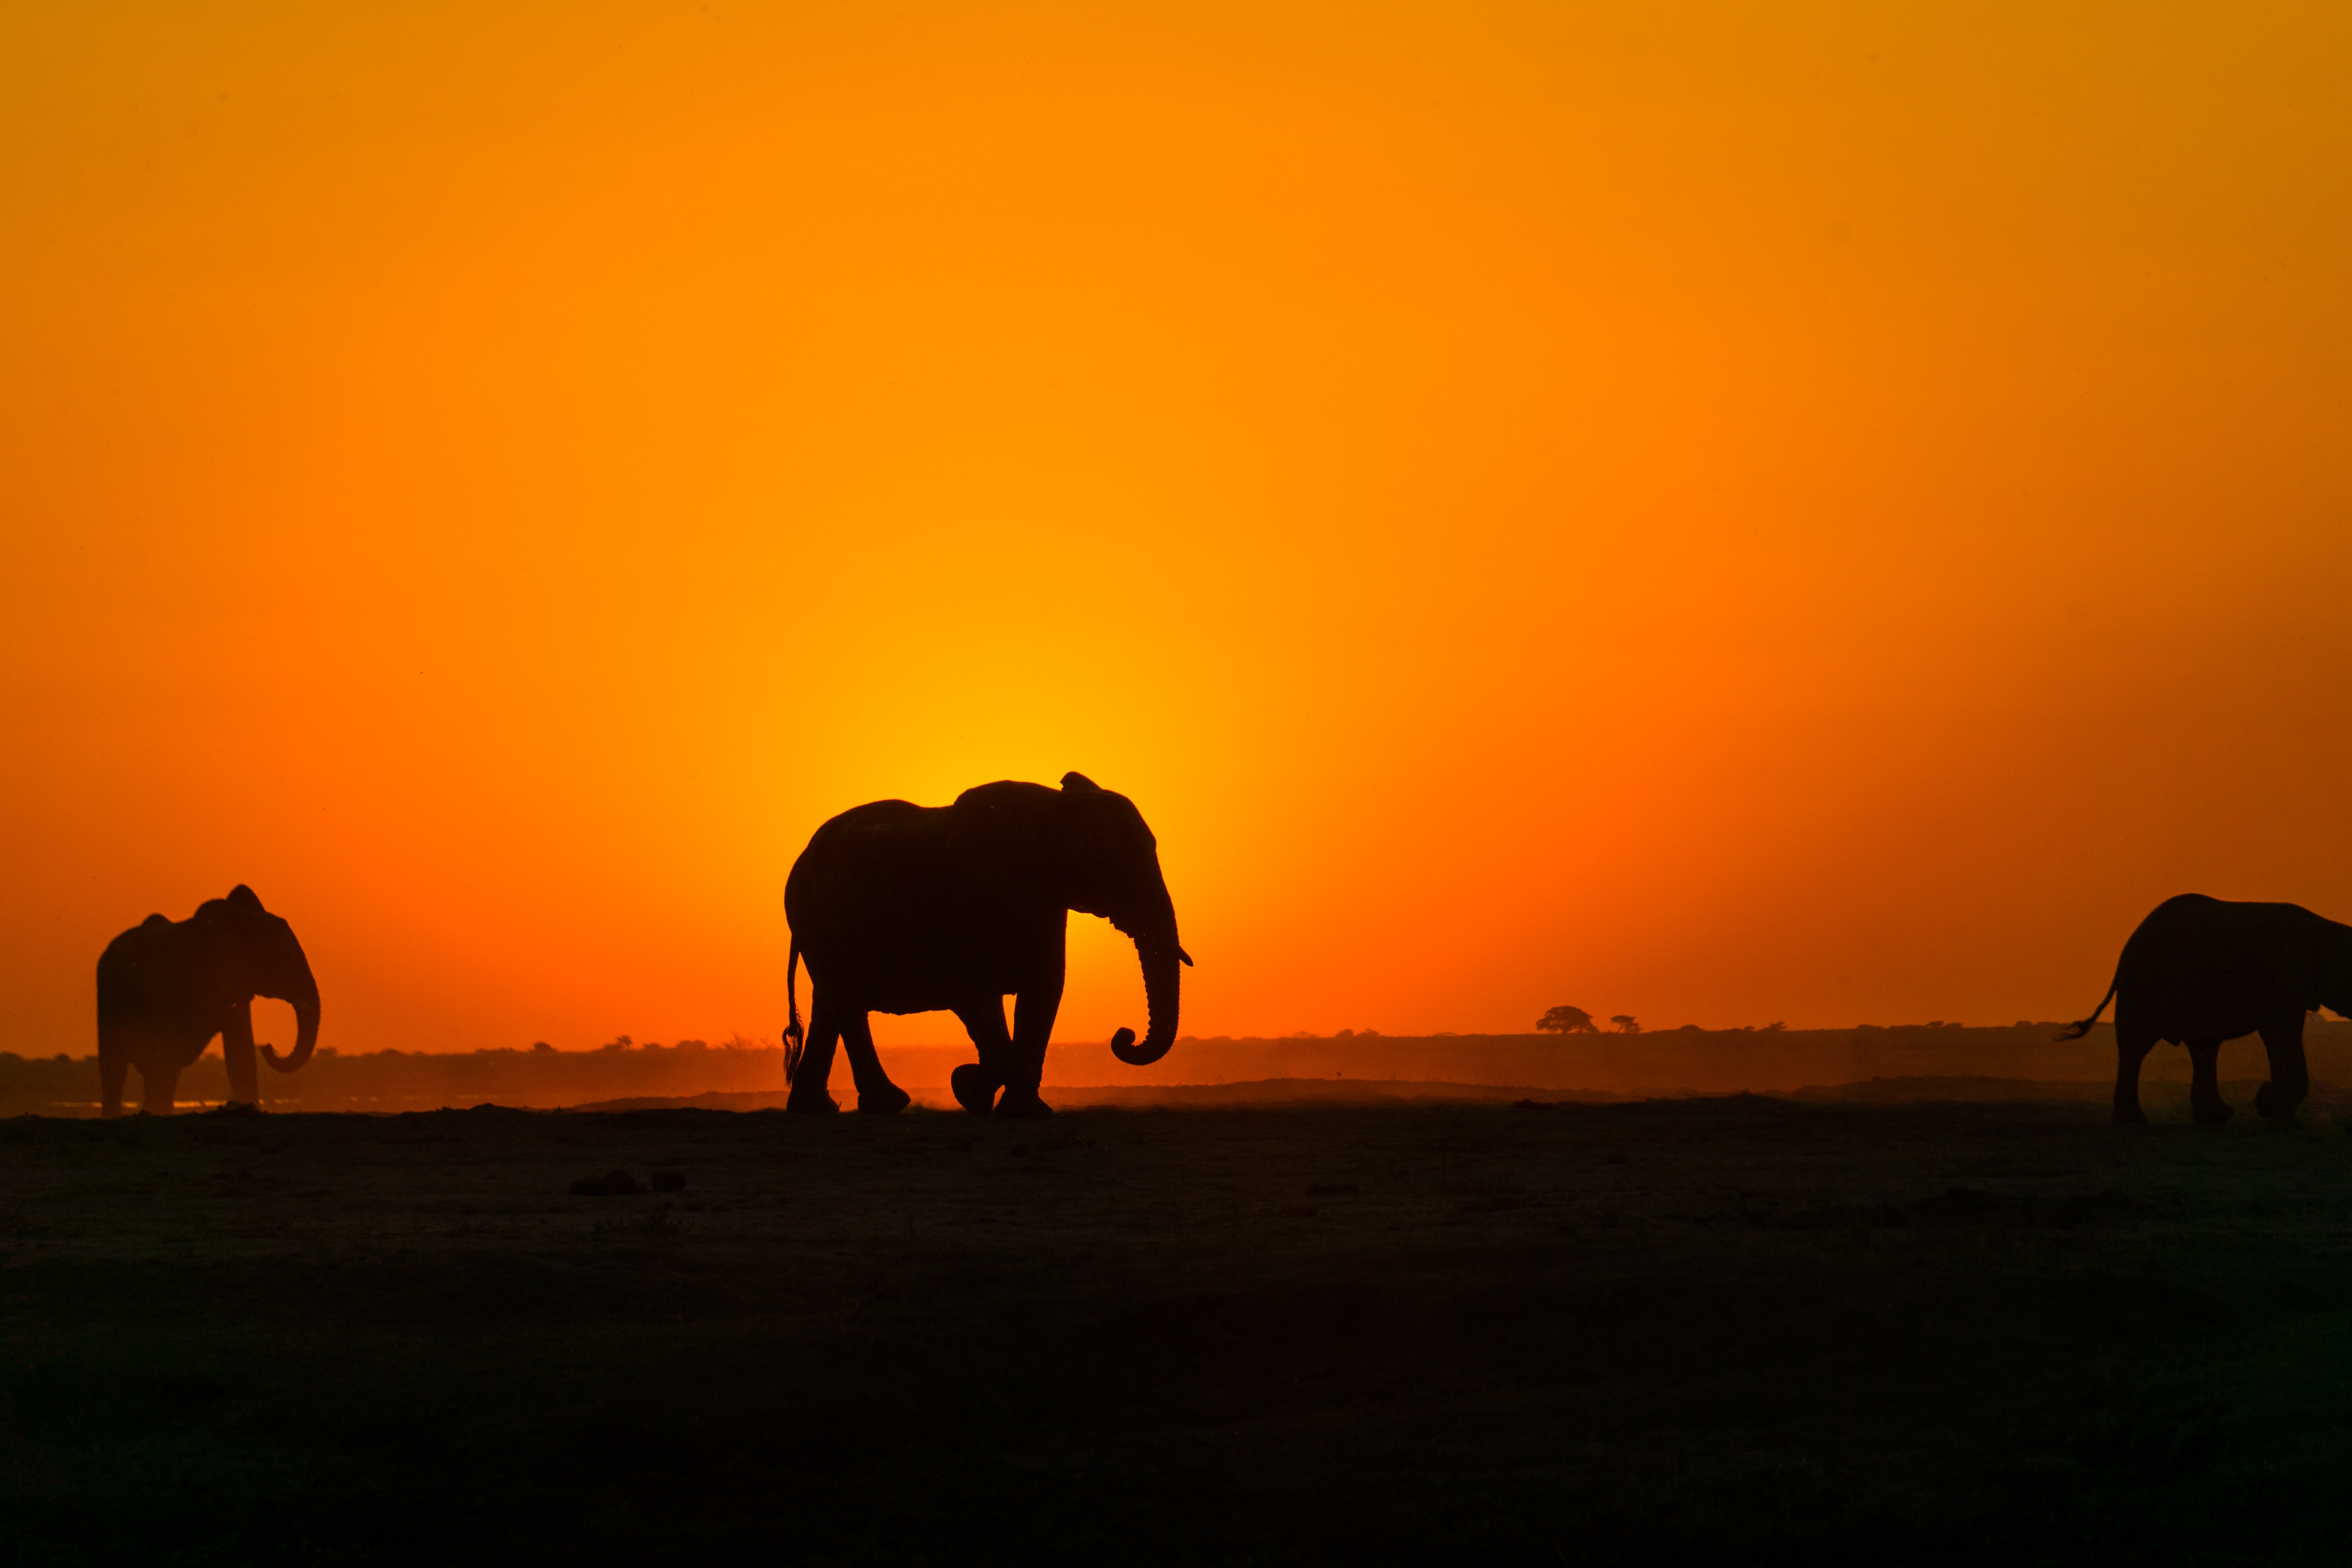
\includegraphics{elephant.jpg}

}

\caption{A full screen image}

\end{figure}%%
\end{figure*}%

Dodatkowo szerokości

\begin{Shaded}
\begin{Highlighting}[]
\NormalTok{knitr}\SpecialCharTok{::}\FunctionTok{kable}\NormalTok{(}
\NormalTok{  mtcars[}\DecValTok{1}\SpecialCharTok{:}\DecValTok{6}\NormalTok{, }\DecValTok{1}\SpecialCharTok{:}\DecValTok{10}\NormalTok{]}
\NormalTok{)}
\end{Highlighting}
\end{Shaded}

\begin{table*}

\begin{tabular}{lrrrrrrrrrr}
\toprule
 & mpg & cyl & disp & hp & drat & wt & qsec & vs & am & gear\\
\midrule
Mazda RX4 & 21.0 & 6 & 160 & 110 & 3.90 & 2.620 & 16.46 & 0 & 1 & 4\\
Mazda RX4
Wag & 21.0 & 6 & 160 & 110 & 3.90 & 2.875 & 17.02 & 0 & 1 & 4\\
Datsun 710 & 22.8 & 4 & 108 & 93 & 3.85 & 2.320 & 18.61 & 1 & 1 & 4\\
Hornet 4
Drive & 21.4 & 6 & 258 & 110 & 3.08 & 3.215 & 19.44 & 1 & 0 & 3\\
Hornet
Sportabout & 18.7 & 8 & 360 & 175 & 3.15 & 3.440 & 17.02 & 0 & 0 & 3\\
Valiant & 18.1 & 6 & 225 & 105 & 2.76 & 3.460 & 20.22 & 1 & 0 & 3\\
\bottomrule
\end{tabular}

\end{table*}%

\section{Koniec dokumentu}\label{koniec}

\subsection{Koniec strony}\label{koniec-strony}

Przed przerwą

\newpage{}

Umieszczamy informacje takie a takie

\bookmarksetup{startatroot}

\chapter{Document - Sample 1}\label{document---sample-1}

Software Requirements Specification

\begin{enumerate}
\def\labelenumi{\arabic{enumi}.}
\setcounter{enumi}{-1}
\item
  Metryka

  \begin{enumerate}
  \def\labelenumii{\arabic{enumii}.}
  \tightlist
  \item
    Tytuł
  \item
    Logo/ Unikalny numer / Wersja dokumentu (wersja z Github?)
  \item
    Data utworzenia / Data modyfikacji
  \item
    Authors (Tabela: Name, Role, Department)
  \item
    Historia dokumentu (Tabela: Data, Wersja, Revision Description,
    Revision Author)
  \item
    Approvals (może na końcu tabela: Approval date, Approved Version,
    Approver Role, Approver)
  \end{enumerate}
\item
  Introduction

  \begin{enumerate}
  \def\labelenumii{\arabic{enumii}.}
  \tightlist
  \item
    Cel projektu (purpose of project)
  \item
    Definicje, akronimy, skróty, słownik (Terms, Acronyms and
    Definitions)
  \item
    Odnośniki i powiązane dokumenty (Related documents)
  \item
    Instrukcja obsługi (opcja)
  \end{enumerate}
\item
  Opis systemu

  \begin{enumerate}
  \def\labelenumii{\arabic{enumii}.}
  \tightlist
  \item
    Zakres (Scope)

    \begin{enumerate}
    \def\labelenumiii{\arabic{enumiii}.}
    \tightlist
    \item
      Funkcjonalności z zakresie (In Scope Functionality)
    \item
      Poza zakresem (Out of Scope Functionality)
    \end{enumerate}
  \item
    Kontekst systemu - Opis systemu, jak system będzie wpasowany w
    otoczenie, interakcje z innymi systemami
  \item
  \end{enumerate}
\item
  Goals
\item
  Functional Requirements
\item
  Non-functional requirements
\item
  User Stories
\item
  Wireframes
\item
  Acceptance Criteria
\item
  Rules
\item
  Assumptions and Constraints
\end{enumerate}

RACI? co jeszcze, tabele - User Stories,

Makiety - opis tabelki do tego,

Lightbox

Test GIT i jak katalog tych dokumentów

\begin{center}\rule{0.5\linewidth}{0.5pt}\end{center}

\bookmarksetup{startatroot}

\chapter{Tables}\label{tables}

\section{Tables}\label{tables-1}

Poniżej znajdują się przykładowe tabele. Zerknij

\subsection{Markdown Tables}\label{markdown-tables}

Ten tekst jest formatowany przez CSS i jest

\begin{longtable}[]{@{}llrc@{}}
\caption{My Caption}\label{tbl-letters}\tabularnewline
\toprule\noalign{}
Default & Left & Right & Center \\
\midrule\noalign{}
\endfirsthead
\toprule\noalign{}
Default & Left & Right & Center \\
\midrule\noalign{}
\endhead
\bottomrule\noalign{}
\endlastfoot
12 & 12 & 12 & 12 \\
123 & 123 & 123 & 123 \\
1 & 1 & 1 & 1 \\
\end{longtable}

When reviewing a document you often want to provide inline comments with
suggested revisions. This is possible in Quarto using HTML comments
(which are ignored by all output formats). Visual mode includes a
command for inserting HTML comments as well as special highlighting
treatment to easily parse out editing comments from surrounding text. No
text.

\section{See}\label{see}

Zobacz tu cross reference -\textgreater{} Table~\ref{tbl-letters}

\textbf{Historia zmian}

\begin{longtable}[]{@{}
  >{\raggedright\arraybackslash}p{(\columnwidth - 6\tabcolsep) * \real{0.1000}}
  >{\centering\arraybackslash}p{(\columnwidth - 6\tabcolsep) * \real{0.1000}}
  >{\raggedright\arraybackslash}p{(\columnwidth - 6\tabcolsep) * \real{0.2000}}
  >{\raggedright\arraybackslash}p{(\columnwidth - 6\tabcolsep) * \real{0.6000}}@{}}
\caption{Historia wersji dokumentu}\label{tbl-ciekawa}\tabularnewline
\toprule\noalign{}
\begin{minipage}[b]{\linewidth}\raggedright
Data zmiany
\end{minipage} & \begin{minipage}[b]{\linewidth}\centering
Wersja dokumentu
\end{minipage} & \begin{minipage}[b]{\linewidth}\raggedright
Kto zmienił
\end{minipage} & \begin{minipage}[b]{\linewidth}\raggedright
Opis zmiany
\end{minipage} \\
\midrule\noalign{}
\endfirsthead
\toprule\noalign{}
\begin{minipage}[b]{\linewidth}\raggedright
Data zmiany
\end{minipage} & \begin{minipage}[b]{\linewidth}\centering
Wersja dokumentu
\end{minipage} & \begin{minipage}[b]{\linewidth}\raggedright
Kto zmienił
\end{minipage} & \begin{minipage}[b]{\linewidth}\raggedright
Opis zmiany
\end{minipage} \\
\midrule\noalign{}
\endhead
\bottomrule\noalign{}
\endlastfoot
08.11.2023 & 1.0 & Michał Lesiowski & Utworzenie dokumentu \\
01.03.2024 & 1.1 & Michał Lesiowski & Aktualizacja - słownik
konfigurator, podgląd zgłoszenia (przycisk edycja), powiadomienia o
akcji \\
06.05.2024 & 1.2 & Michał Lesiowski & Aktualizacja makiet, Baza zgłoszeń
mechanizm edycja/zapisz, dodanie szablonów email do wysyłki informacji z
podglądu zgłoszenia - raport wstępny, raport końcowy. \\
\end{longtable}

Powyższa tabela mogłaby zaciągać informacje z Commit w te miejsca oraz
numery wersji

\bookmarksetup{startatroot}

\chapter{Galery}\label{galery}

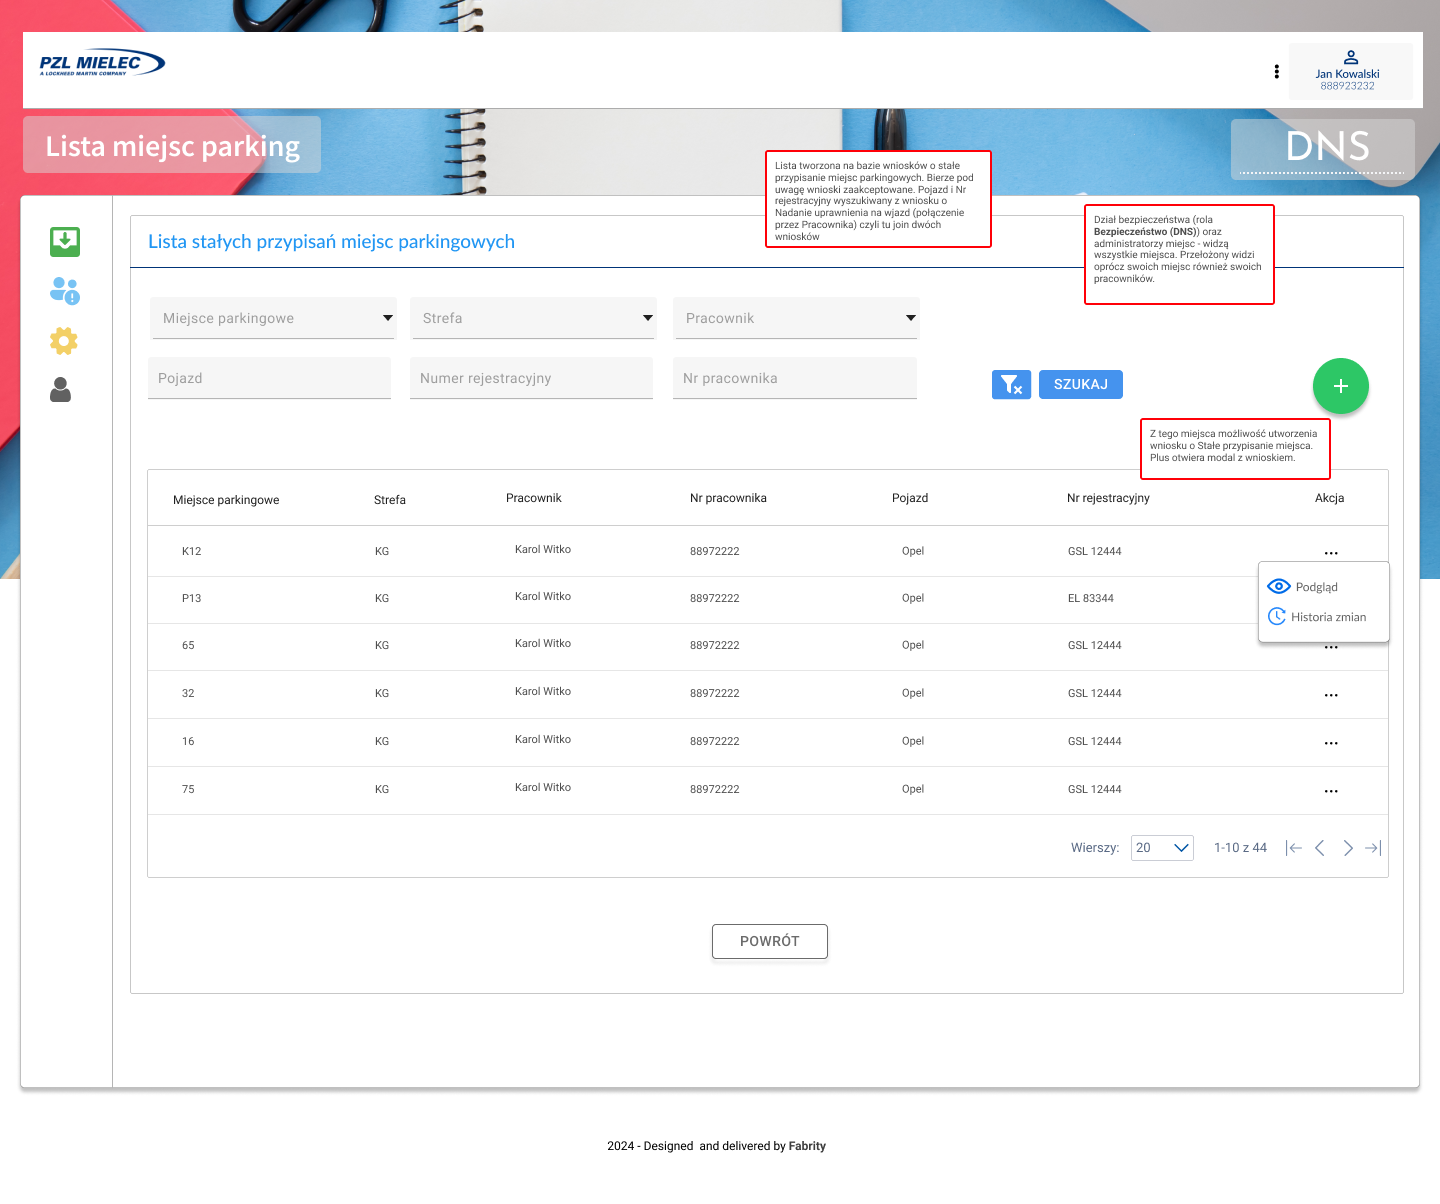
\includegraphics{images/wniosek1.png}\{\#fig-elephant\}

\includegraphics{images/wniosek2.png}
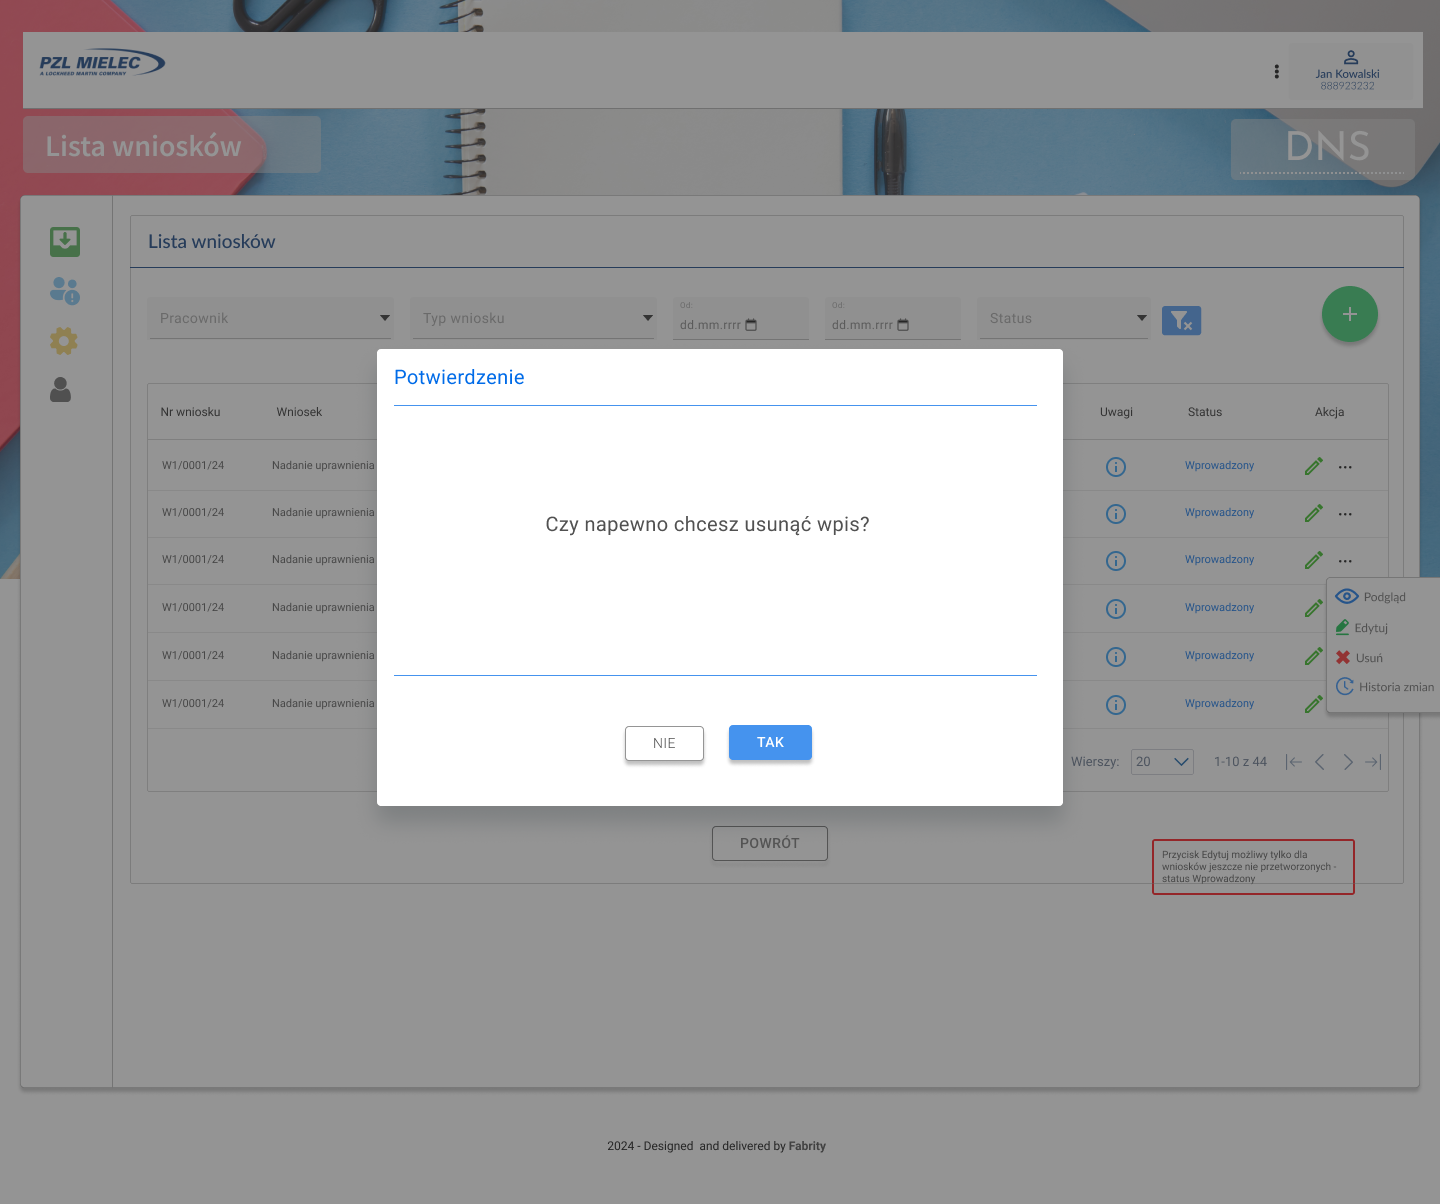
\includegraphics{images/wniosek3.png}

\bookmarksetup{startatroot}

\chapter{Example Lightbox Document}\label{example-lightbox-document}

\section{Chilmark}\label{chilmark}

Here is a simple image with a description. This also overrides the
description position and places it to the left of the image.

\begin{figure}[H]

{\centering 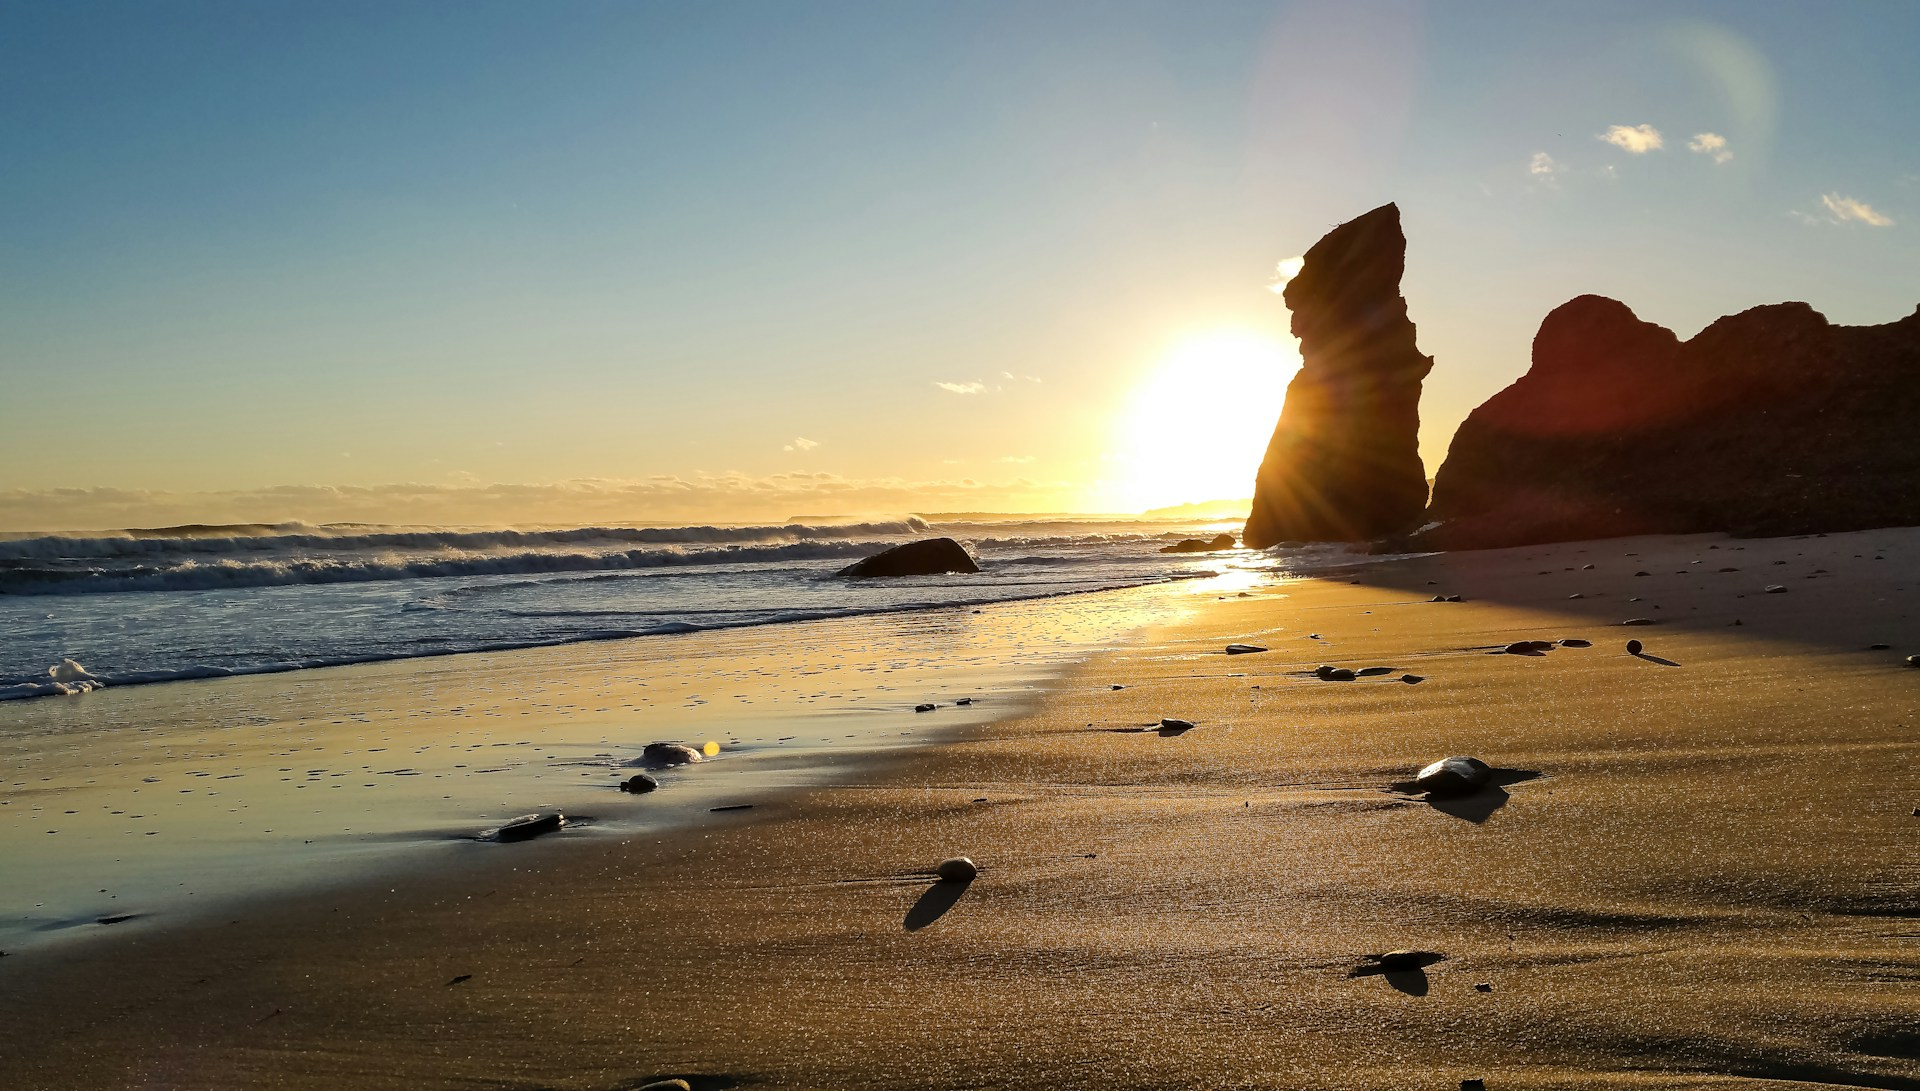
\includegraphics{images/mv-0.jpg}

}

\caption{Beach in Chilmark}

\end{figure}%

\section{Elsewhere}\label{elsewhere}

The below demonstrates placing more than one image in a gallery. Note
the usage of the \texttt{layout-ncol} which arranges the images on the
page side by date. Adding the \texttt{group} attribute to the markdown
images places the images in a gallery grouped together based upon the
group name provided.

\begin{figure}

\begin{minipage}{0.50\linewidth}

\begin{figure}[H]

{\centering 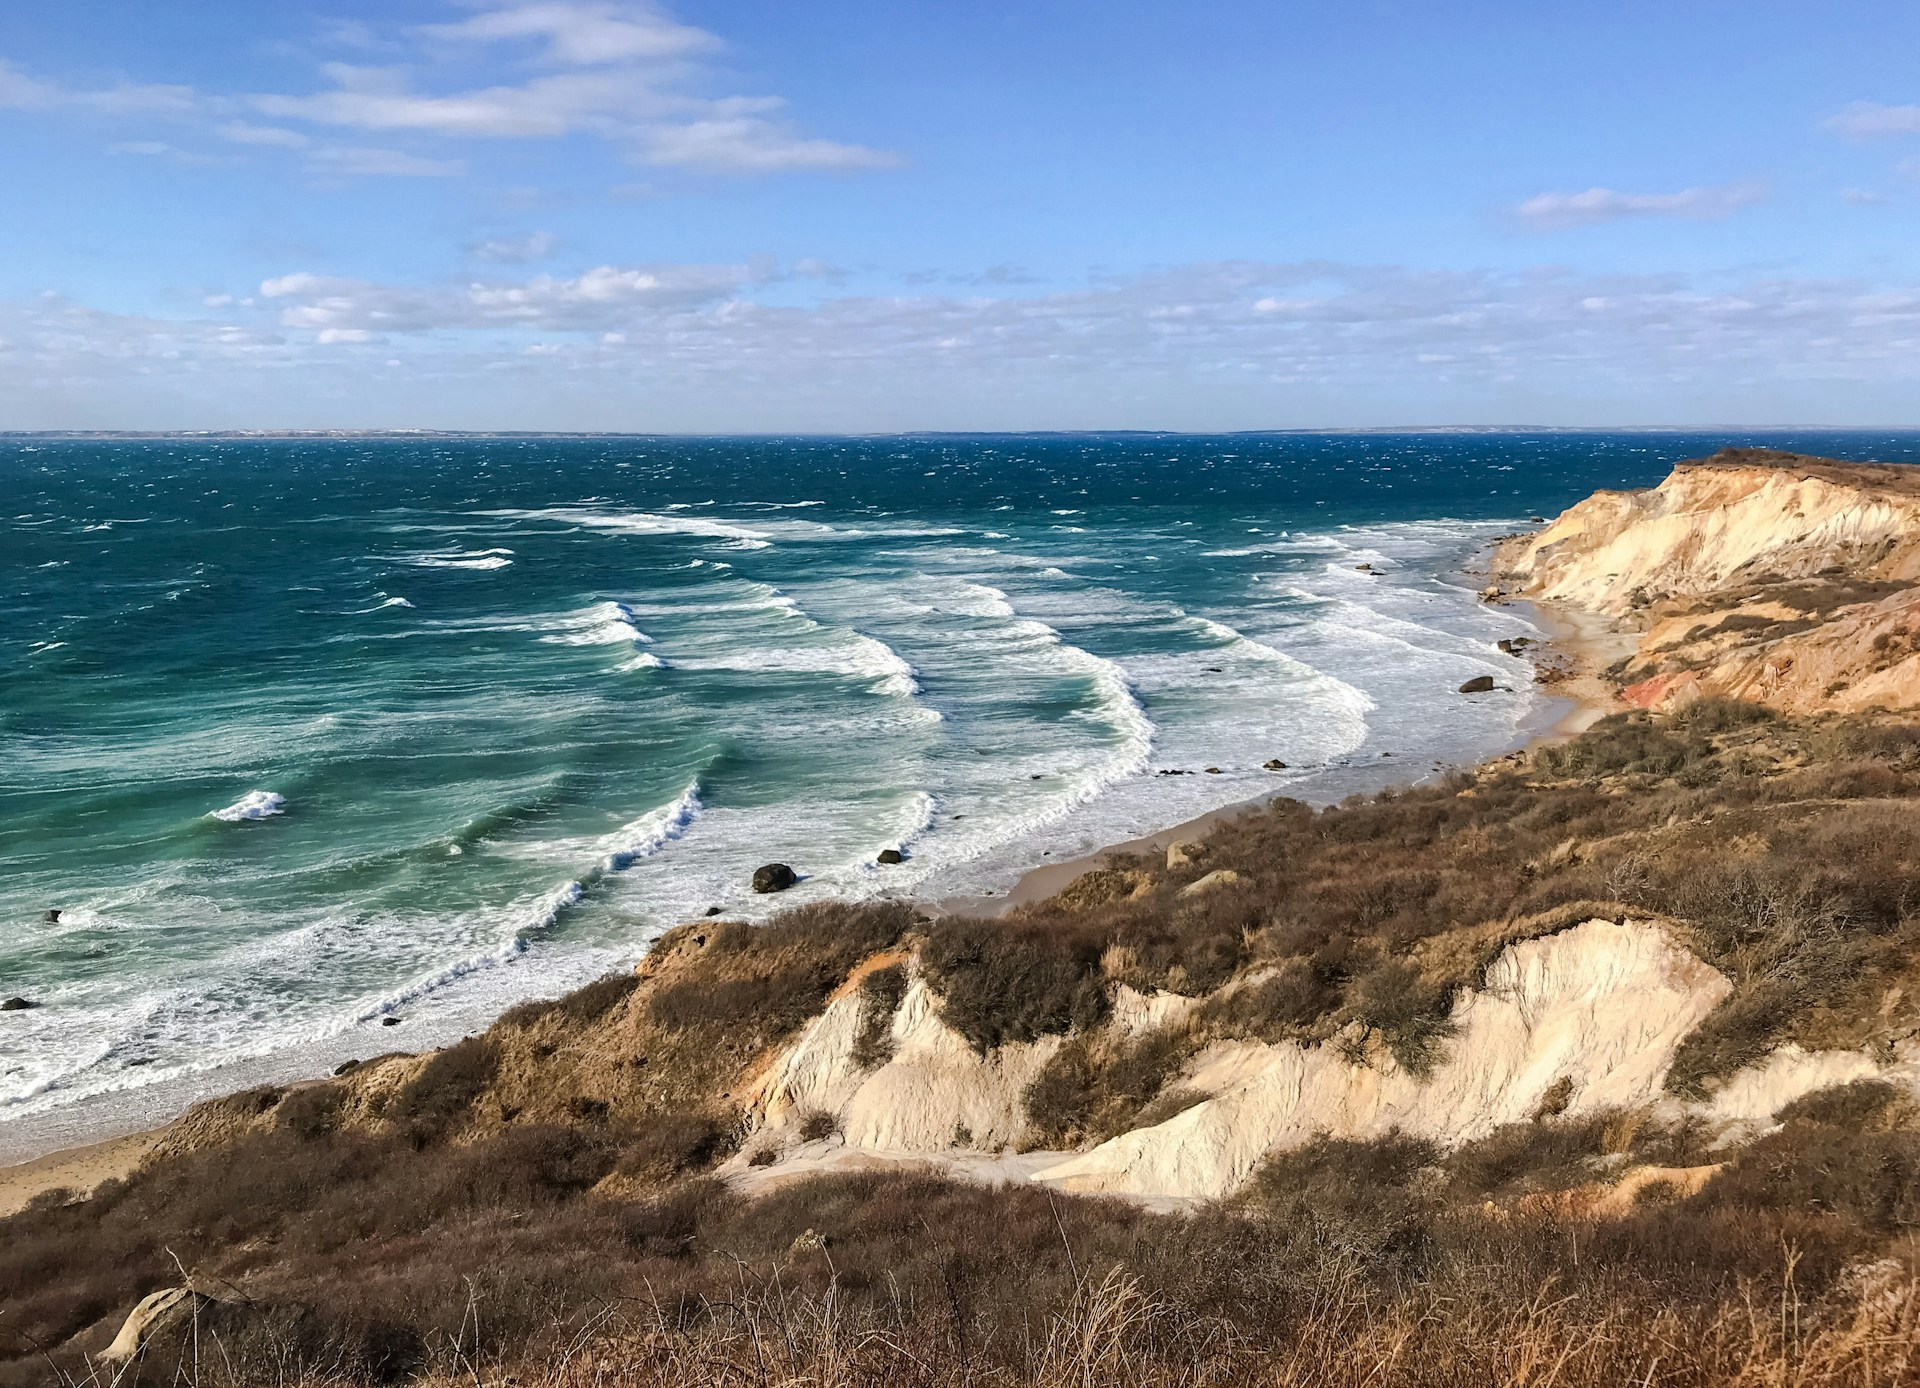
\includegraphics{images/mv-1.jpg}

}

\subcaption{Aquinnah}

\end{figure}%

\end{minipage}%
%
\begin{minipage}{0.50\linewidth}

\begin{figure}[H]

{\centering 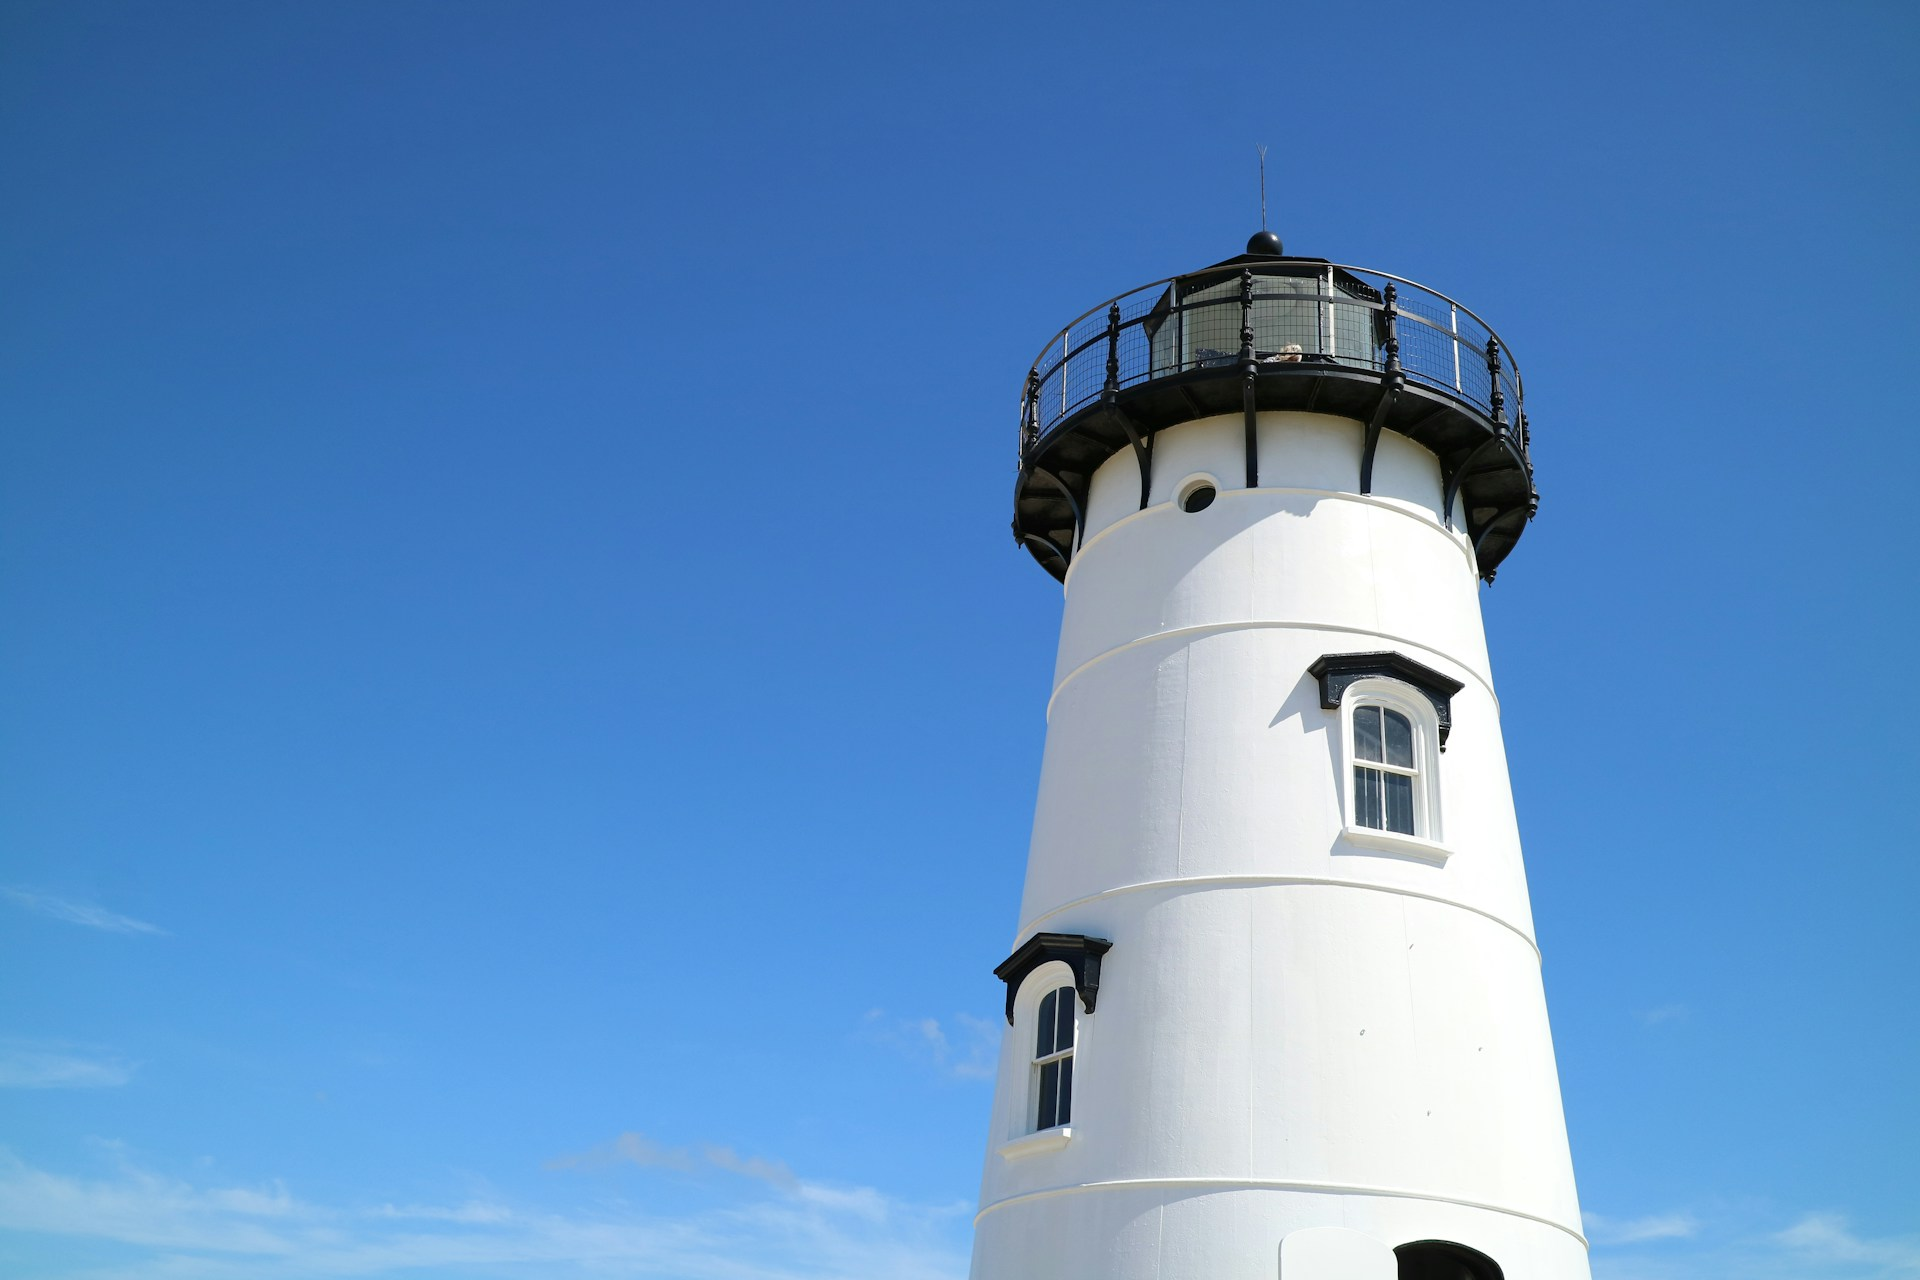
\includegraphics{images/mv-3.jpg}

}

\subcaption{Oak Bluffs}

\end{figure}%

\end{minipage}%
\newline
\begin{minipage}{\linewidth}

\begin{figure}[H]

{\centering 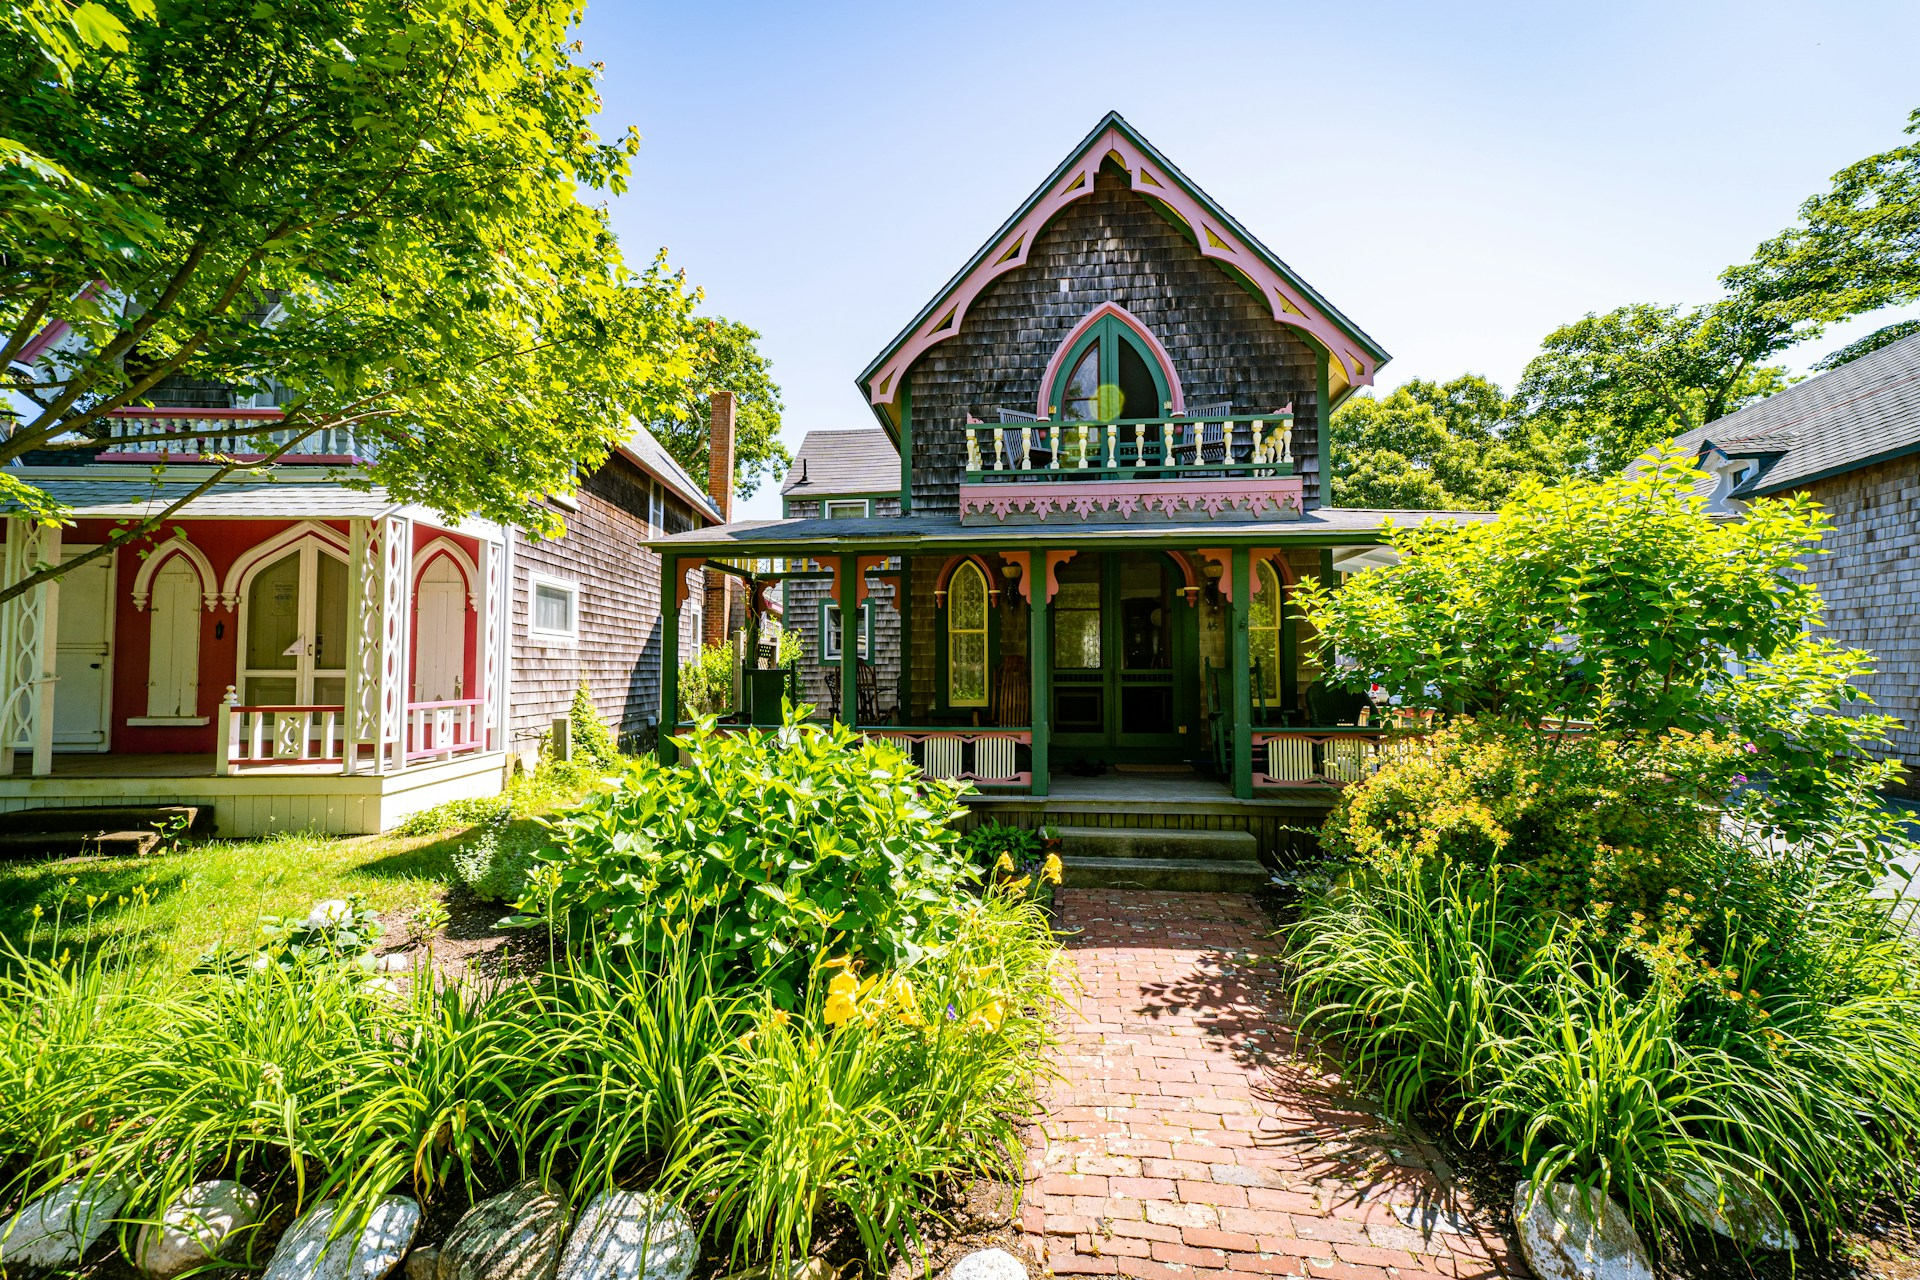
\includegraphics{images/mv-2.jpg}

}

\subcaption{Vineyard lighthouse}

\end{figure}%

\end{minipage}%

\end{figure}%

\section{With computation code
chunks}\label{with-computation-code-chunks}

Options for lightbox can be passed using chunk options.

\begin{Shaded}
\begin{Highlighting}[]
\FunctionTok{plot}\NormalTok{(}\DecValTok{1}\SpecialCharTok{:}\DecValTok{10}\NormalTok{, }\FunctionTok{rnorm}\NormalTok{(}\DecValTok{10}\NormalTok{))}
\end{Highlighting}
\end{Shaded}

\begin{figure}[H]

{\centering 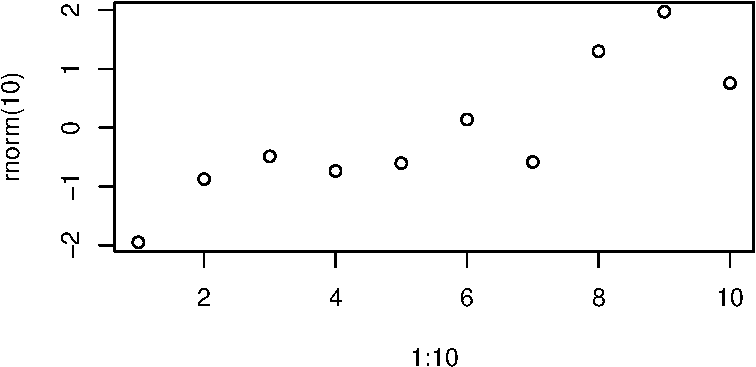
\includegraphics{lightbox_files/figure-pdf/unnamed-chunk-1-1.pdf}

}

\caption{Simple demo R plot}

\end{figure}%

\begin{Shaded}
\begin{Highlighting}[]
\FunctionTok{plot}\NormalTok{(cars)}
\end{Highlighting}
\end{Shaded}

\begin{figure}[H]

{\centering 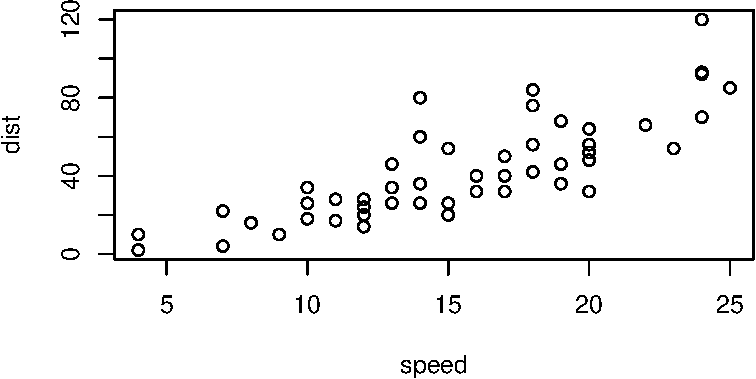
\includegraphics{lightbox_files/figure-pdf/unnamed-chunk-2-1.pdf}

}

\caption{Plot about cars data}

\end{figure}%

It is possible to create several plots, and group them in a lightbox
gallery. Use list in YAML for options when you have several plots, on
per plot.

\begin{Shaded}
\begin{Highlighting}[]
\FunctionTok{plot}\NormalTok{(mtcars)}
\end{Highlighting}
\end{Shaded}

\begin{figure}[H]

{\centering 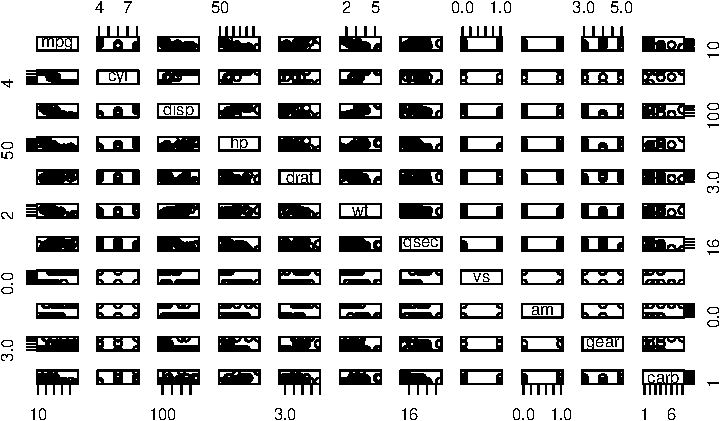
\includegraphics{lightbox_files/figure-pdf/unnamed-chunk-3-1.pdf}

}

\caption{Caption for first plot}

\end{figure}%

\begin{Shaded}
\begin{Highlighting}[]
\FunctionTok{plot}\NormalTok{(cars)}
\end{Highlighting}
\end{Shaded}

\begin{figure}[H]

{\centering 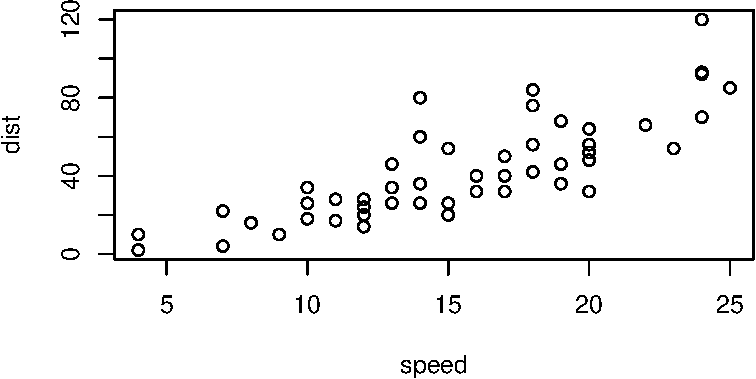
\includegraphics{lightbox_files/figure-pdf/unnamed-chunk-3-2.pdf}

}

\caption{Caption for second plot}

\end{figure}%

When \texttt{lightbox:\ auto} in main YAML config, you can opt-out
lightbox on a plot by setting \texttt{lightbox:\ false}

\begin{Shaded}
\begin{Highlighting}[]
\FunctionTok{plot}\NormalTok{(mtcars)}
\end{Highlighting}
\end{Shaded}

\begin{figure}[H]

{\centering 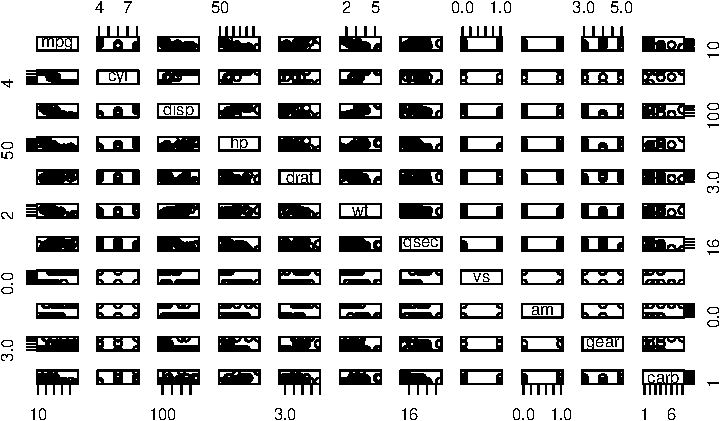
\includegraphics{lightbox_files/figure-pdf/unnamed-chunk-4-1.pdf}

}

\caption{mtcars}

\end{figure}%

\section{Credits}\label{credits}

The images in this example were used under the
\href{https://unsplash.com/license}{Unsplash license}, view originals
below:

\begin{itemize}
\tightlist
\item
  \href{https://unsplash.com/photos/VBDJGOMCwps}{Chilmark Beach}
\item
  \href{https://unsplash.com/photos/2iQnDPLIXwU}{Aquinnah}
\item
  \href{https://unsplash.com/photos/HQEtvlNzUyA}{Gingerbread House}
\item
  \href{https://unsplash.com/photos/f59MyOfLpi8}{Edgartown Light}
\item
  \href{https://unsplash.com/photos/IiLiz7XpQpI}{Edgartown Sailboat}
\end{itemize}

\bookmarksetup{startatroot}

\chapter{\_Przykłady elementów}\label{przykux142ady-elementuxf3w}

Poniżej elementy do zastosowania w DSP.

\section{Formatowanie}\label{formatowanie}

\begin{itemize}
\tightlist
\item
  \textbf{Verbatim code}
\end{itemize}


\includegraphics[width=5.375in,height=\textheight]{images/_format_verbatim.png}

\texttt{Tu\ jest\ verbatim\ code}

\begin{center}\rule{0.5\linewidth}{0.5pt}\end{center}

\begin{itemize}
\tightlist
\item
  \textbf{Term definition}
\end{itemize}

\begin{description}
\item[Term 1]
definicja terminu
\end{description}

\begin{center}\rule{0.5\linewidth}{0.5pt}\end{center}

\begin{itemize}
\tightlist
\item
  \textbf{Block quotes}
\end{itemize}


\includegraphics[width=4.97917in,height=\textheight]{images/clipboard-169377371.png}

\begin{quote}
To jest block quotes
\end{quote}

\begin{center}\rule{0.5\linewidth}{0.5pt}\end{center}

\begin{itemize}
\tightlist
\item
  \textbf{HTML własny np. odstępy}
\end{itemize}

\texttt{\textless{}div\ style="margin-top:\ 30px;"\textgreater{}\textless{}/div\textgreater{}}

\begin{center}\rule{0.5\linewidth}{0.5pt}\end{center}

\begin{itemize}
\tightlist
\item
  \textbf{Podświetlenie tekstu mark}
\end{itemize}

\texttt{\textless{}mark\textgreater{}\ To\ jest\ zmarkowany\ tekst\ \textless{}/mark\textgreater{}}

\begin{center}\rule{0.5\linewidth}{0.5pt}\end{center}

\begin{itemize}
\tightlist
\item
  \textbf{Ukrycie elementu}
\end{itemize}


\includegraphics[width=4.40625in,height=\textheight]{images/_format_hidden.png}

\begin{center}\rule{0.5\linewidth}{0.5pt}\end{center}

\section{Callouts}\label{callouts}

\begin{itemize}
\tightlist
\item
  \textbf{Podstawowe callouts}
\end{itemize}

\begin{tcolorbox}[enhanced jigsaw, bottomrule=.15mm, titlerule=0mm, colbacktitle=quarto-callout-caution-color!10!white, coltitle=black, rightrule=.15mm, opacitybacktitle=0.6, colframe=quarto-callout-caution-color-frame, colback=white, breakable, arc=.35mm, toptitle=1mm, leftrule=.75mm, bottomtitle=1mm, title=\textcolor{quarto-callout-caution-color}{\faFire}\hspace{0.5em}{Caution}, toprule=.15mm, left=2mm, opacityback=0]

Tu znajduje się zwijana sekcja w boxie callout typu caution

\end{tcolorbox}


\includegraphics{images/_format_call1.png}

\begin{tcolorbox}[enhanced jigsaw, bottomrule=.15mm, titlerule=0mm, colbacktitle=quarto-callout-tip-color!10!white, coltitle=black, rightrule=.15mm, opacitybacktitle=0.6, colframe=quarto-callout-tip-color-frame, colback=white, breakable, arc=.35mm, toptitle=1mm, leftrule=.75mm, bottomtitle=1mm, title=\textcolor{quarto-callout-tip-color}{\faLightbulb}\hspace{0.5em}{Tip}, toprule=.15mm, left=2mm, opacityback=0]

Altair is based on Vega-Lite, a high-level grammar of interactive
graphics

\end{tcolorbox}


\includegraphics{images/_format_call2.png}

\begin{tcolorbox}[enhanced jigsaw, bottomrule=.15mm, titlerule=0mm, colbacktitle=quarto-callout-note-color!10!white, coltitle=black, rightrule=.15mm, opacitybacktitle=0.6, colframe=quarto-callout-note-color-frame, colback=white, breakable, arc=.35mm, toptitle=1mm, leftrule=.75mm, bottomtitle=1mm, title=\textcolor{quarto-callout-note-color}{\faInfo}\hspace{0.5em}{Note}, toprule=.15mm, left=2mm, opacityback=0]

A tu znajduje się callout note

\end{tcolorbox}


\includegraphics{images/_format_call3.png}

\begin{tcolorbox}[enhanced jigsaw, bottomrule=.15mm, titlerule=0mm, colbacktitle=quarto-callout-important-color!10!white, coltitle=black, rightrule=.15mm, opacitybacktitle=0.6, colframe=quarto-callout-important-color-frame, colback=white, breakable, arc=.35mm, toptitle=1mm, leftrule=.75mm, bottomtitle=1mm, title=\textcolor{quarto-callout-important-color}{\faExclamation}\hspace{0.5em}{This is Important}, toprule=.15mm, left=2mm, opacityback=0]

Danger, callouts will really improve your writing.

\end{tcolorbox}

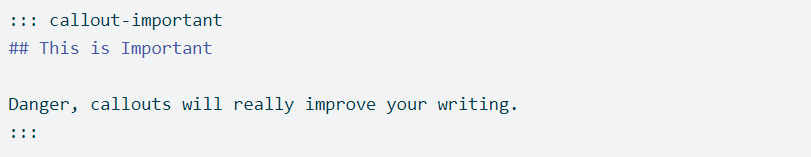
\includegraphics[width=5.20833in,height=\textheight]{images/_format_call4.png}

\begin{center}\rule{0.5\linewidth}{0.5pt}\end{center}

\section{Kolumny}\label{kolumny}

\begin{itemize}
\tightlist
\item
  \textbf{Trzy kolumny}
\end{itemize}

\begin{figure}

\begin{minipage}{0.33\linewidth}
This is a template for a simple Quarto book output to html, PDF or docx
format. It includes a GitHub Action that will build the website
automatically when you make changes to the files.\end{minipage}%
%
\begin{minipage}{0.33\linewidth}
This is a template for a simple Quarto book output to html, PDF or docx
format. It includes a GitHub Action that will build the website
automatically when you make changes to the files.\end{minipage}%
%
\begin{minipage}{0.33\linewidth}
This is a template for a simple Quarto book output to html, PDF or docx
format. It includes a GitHub Action that will build the website
automatically when you make changes to the files.\end{minipage}%

\end{figure}%

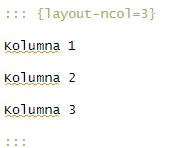
\includegraphics{images/_format_kolumny3.png}

\begin{center}\rule{0.5\linewidth}{0.5pt}\end{center}

\begin{itemize}
\tightlist
\item
  \textbf{Dwie kolumny}
\end{itemize}

This is a template for a simple Quarto book output to html, PDF or docx
format. It includes a GitHub Action that will build the website
automatically when you make changes to the files.

This is a template for a simple Quarto book output to html, PDF or docx
format. It includes a GitHub Action that will build the website
automatically when you make changes to the files.

\begin{center}\rule{0.5\linewidth}{0.5pt}\end{center}

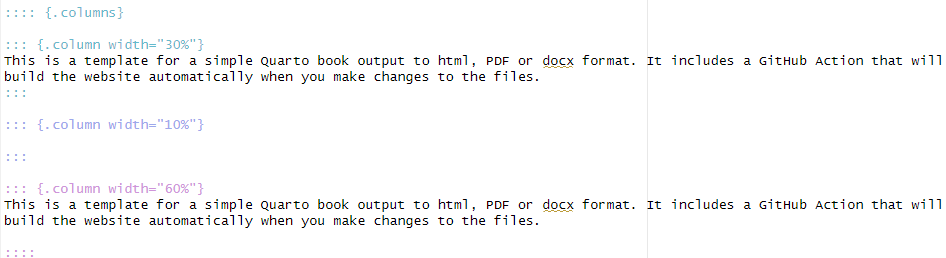
\includegraphics{images/_format_kolumny2.png}

\begin{center}\rule{0.5\linewidth}{0.5pt}\end{center}

\section{Grafiki}\label{grafiki}

\begin{itemize}
\tightlist
\item
  \textbf{Lightbox}
\end{itemize}

\begin{figure}[H]

{\centering 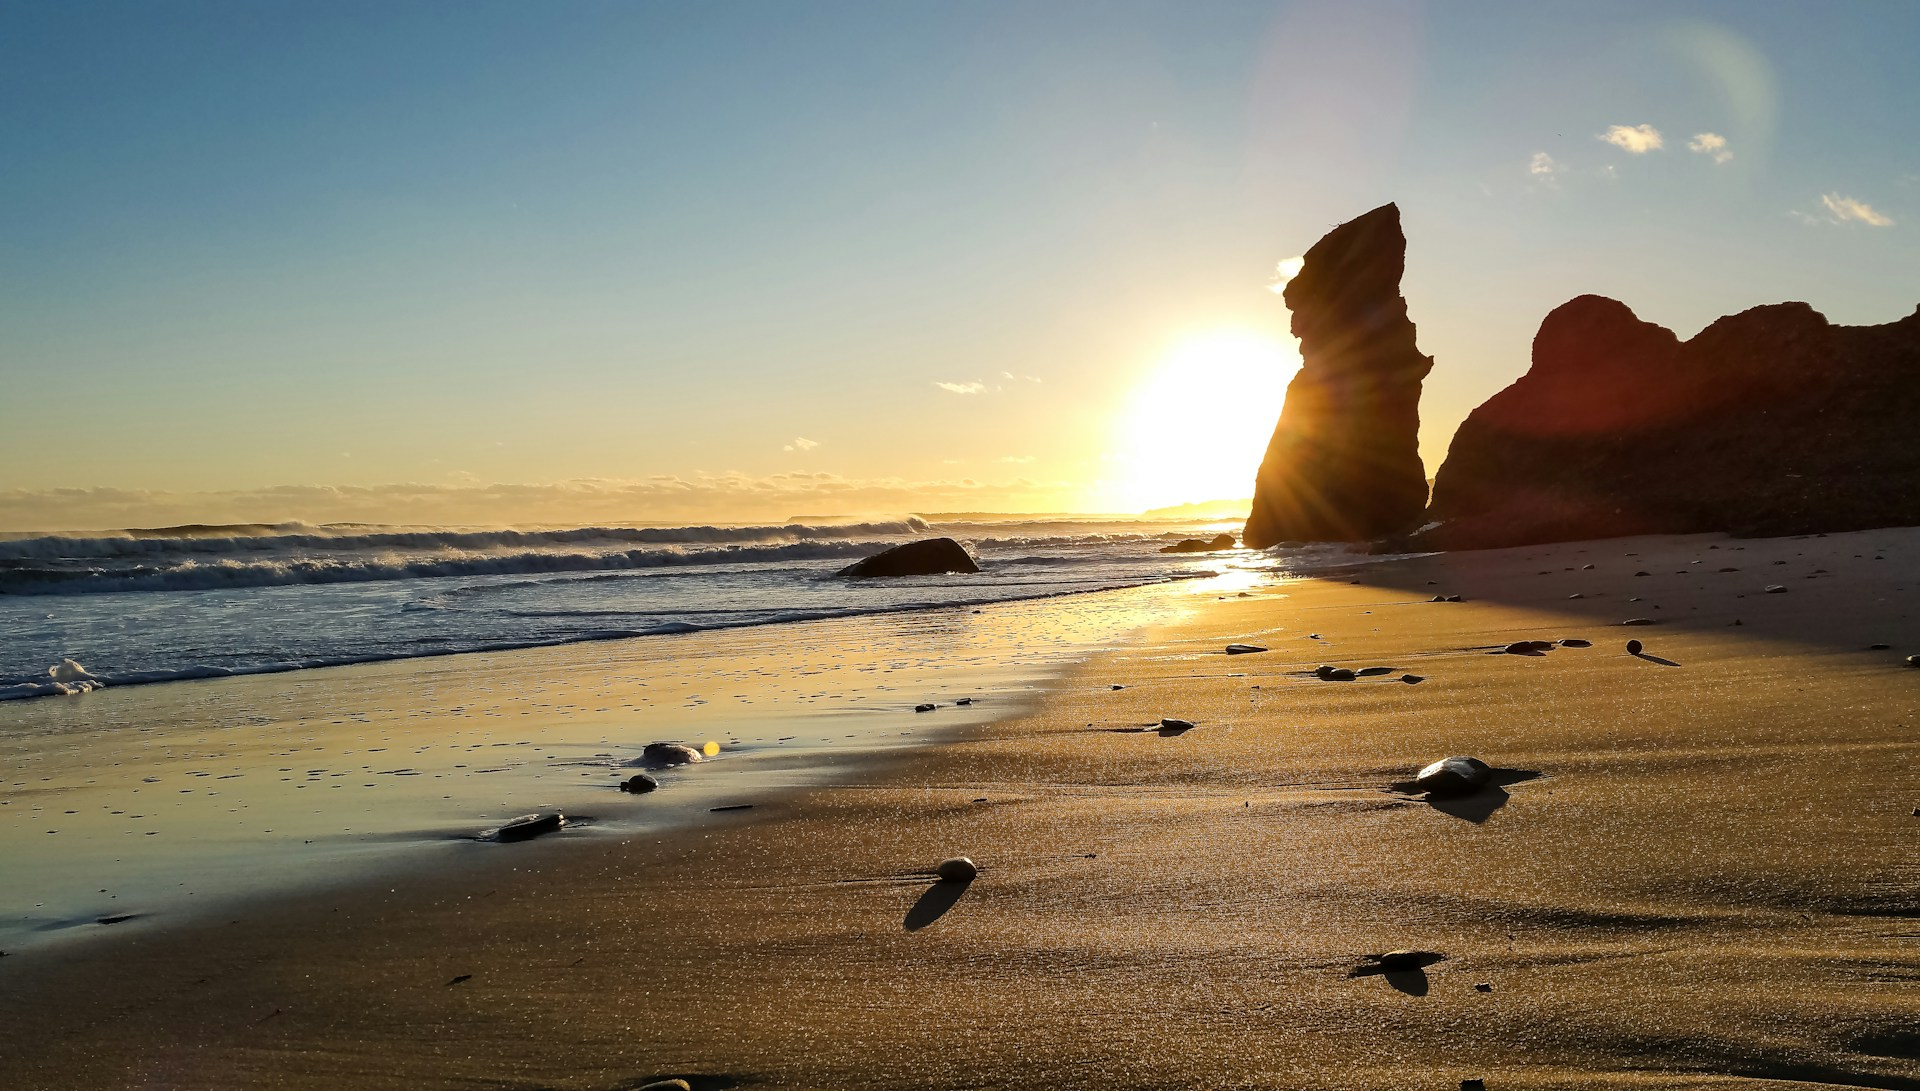
\includegraphics{images/mv-0.jpg}

}

\caption{Beach in Chilmark}

\end{figure}%


\includegraphics{images/_format_lightbox1.png}

\begin{center}\rule{0.5\linewidth}{0.5pt}\end{center}

\begin{itemize}
\tightlist
\item
  \textbf{Lightbox grupa}
\end{itemize}

The below demonstrates placing more than one image in a gallery. Note
the usage of the \texttt{layout-ncol} which arranges the images on the
page side by date. Adding the \texttt{group} attribute to the markdown
images places the images in a gallery grouped together based upon the
group name provided.

\begin{figure}

\begin{minipage}{0.50\linewidth}

\begin{figure}[H]

{\centering 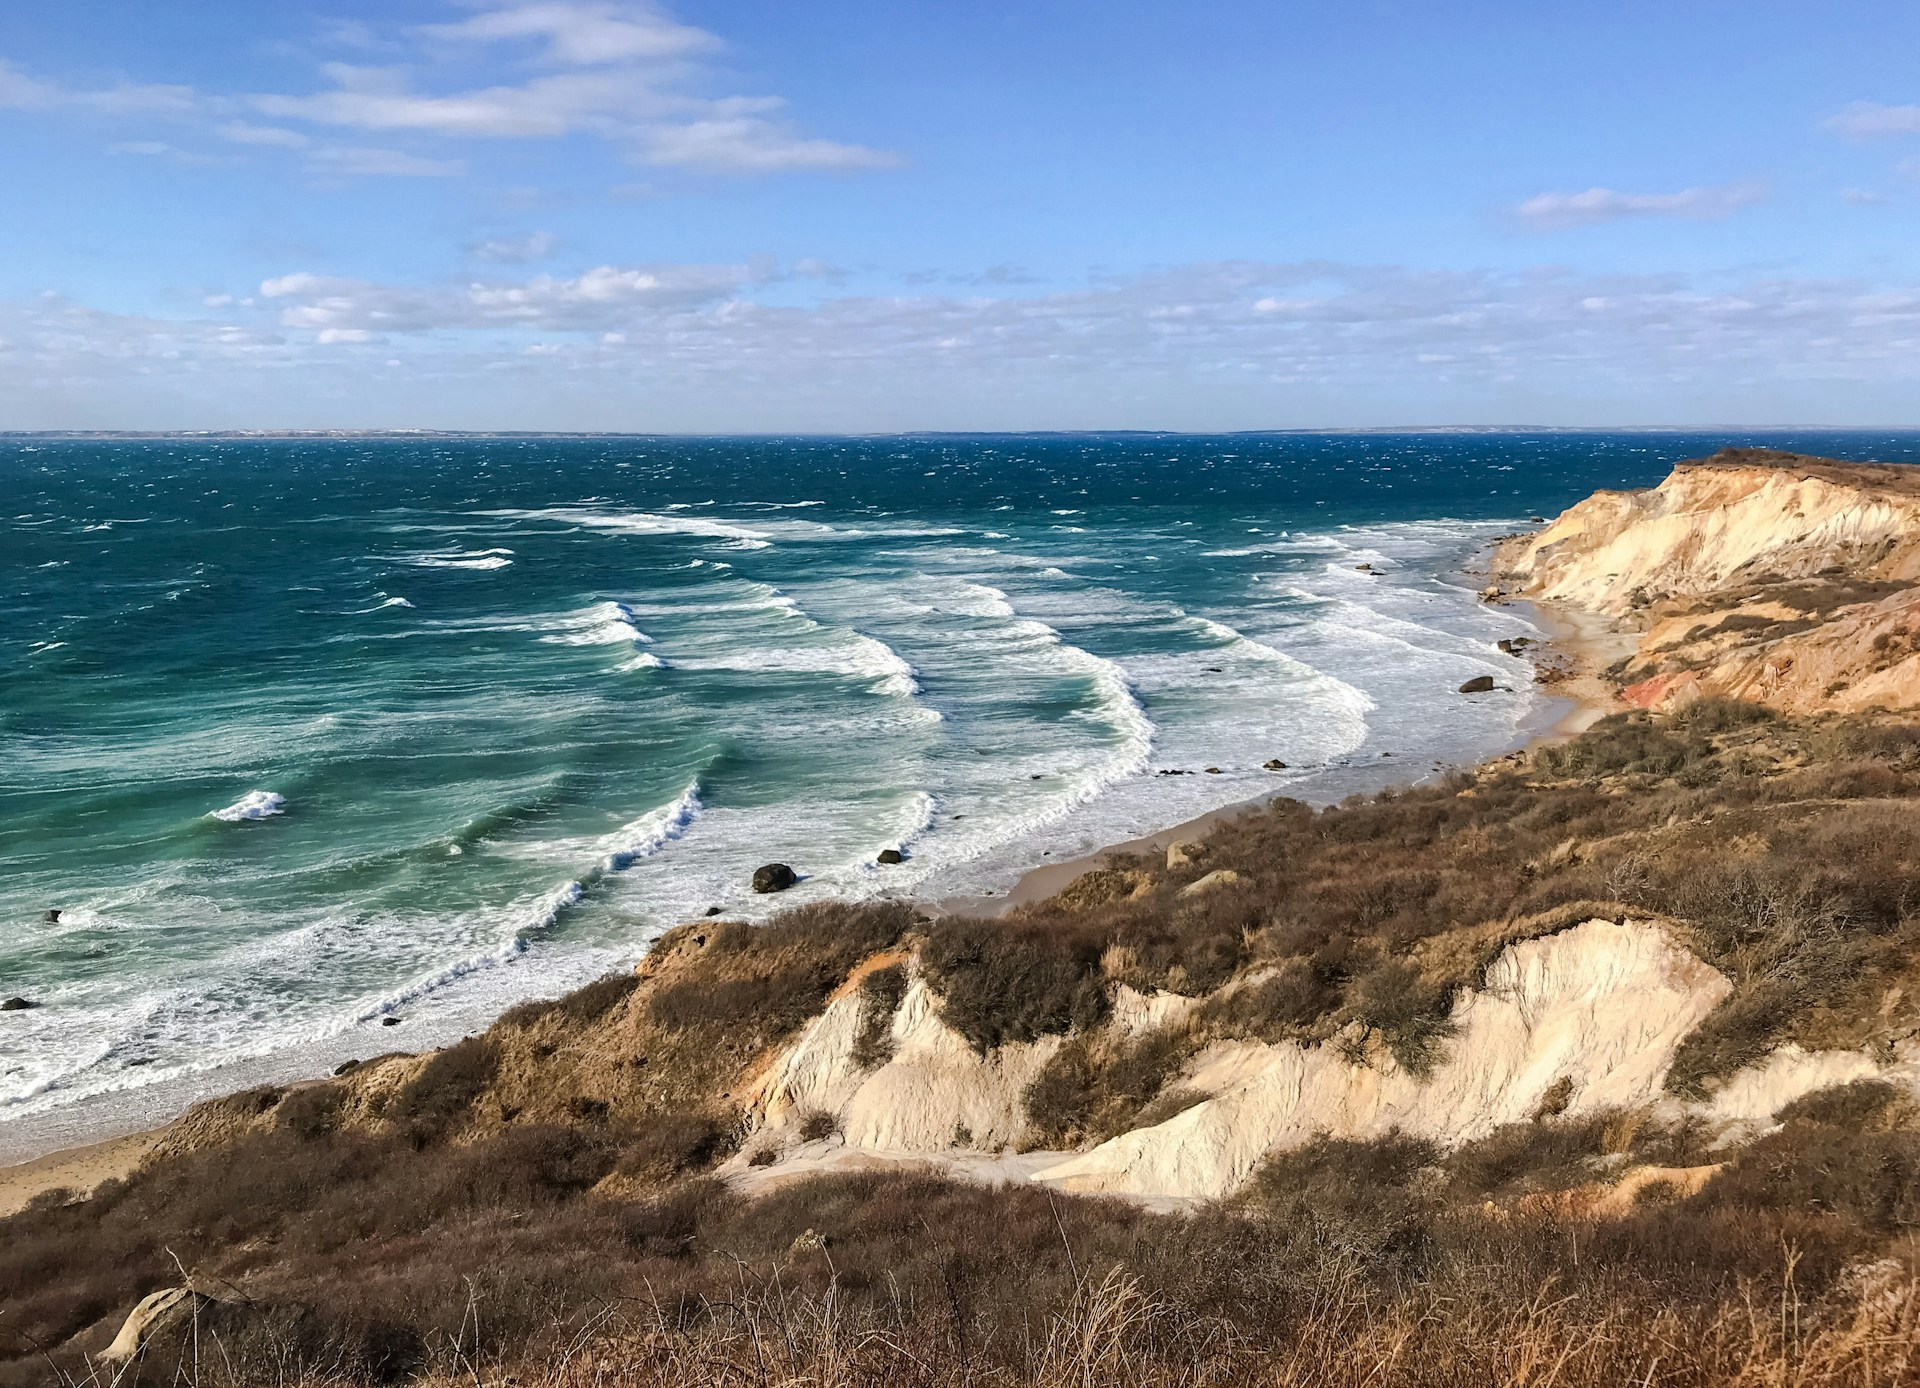
\includegraphics{images/mv-1.jpg}

}

\subcaption{Aquinnah}

\end{figure}%

\end{minipage}%
%
\begin{minipage}{0.50\linewidth}

\begin{figure}[H]

{\centering 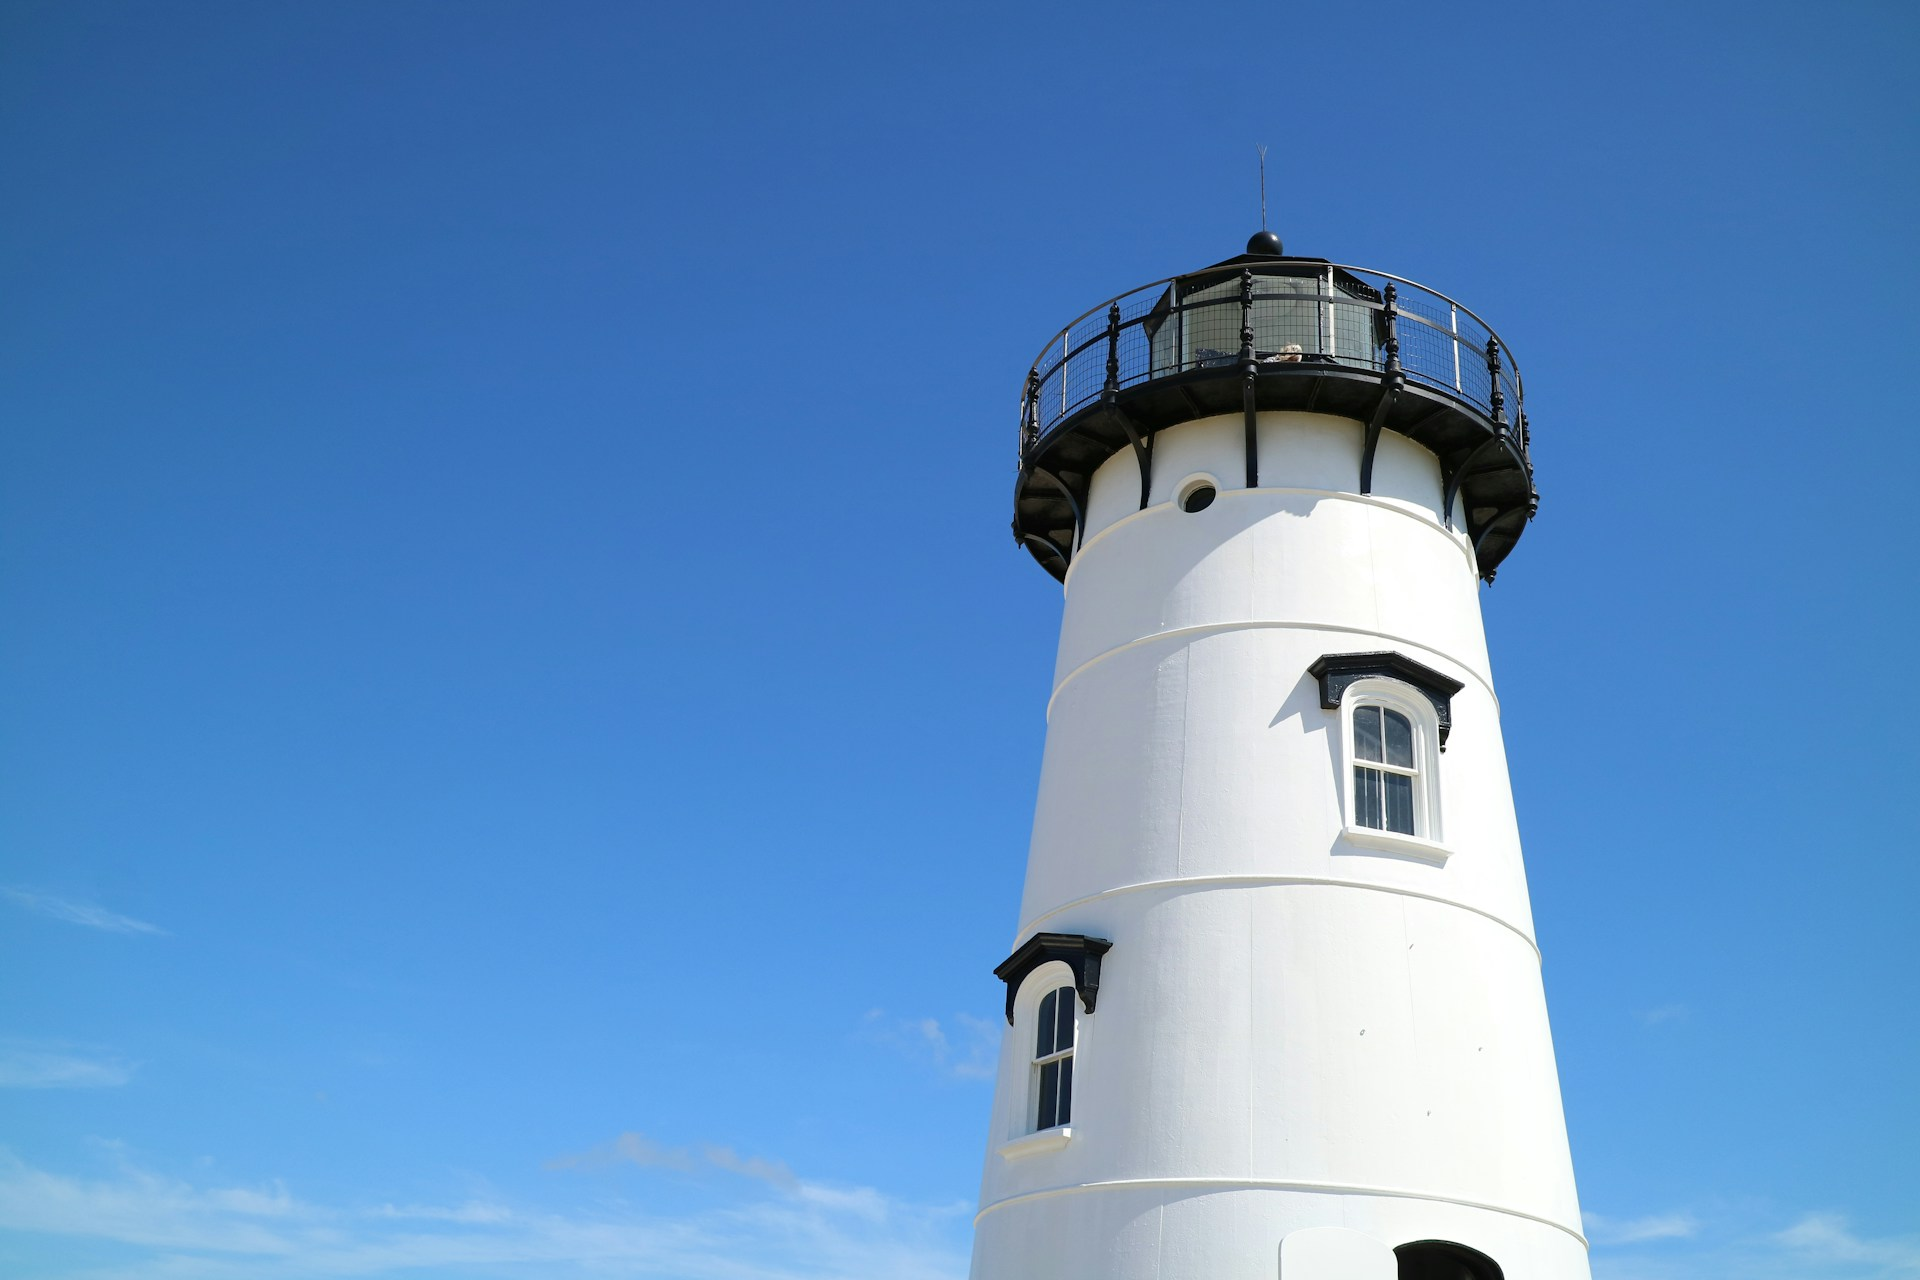
\includegraphics{images/mv-3.jpg}

}

\subcaption{Oak Bluffs}

\end{figure}%

\end{minipage}%
\newline
\begin{minipage}{\linewidth}

\begin{figure}[H]

{\centering 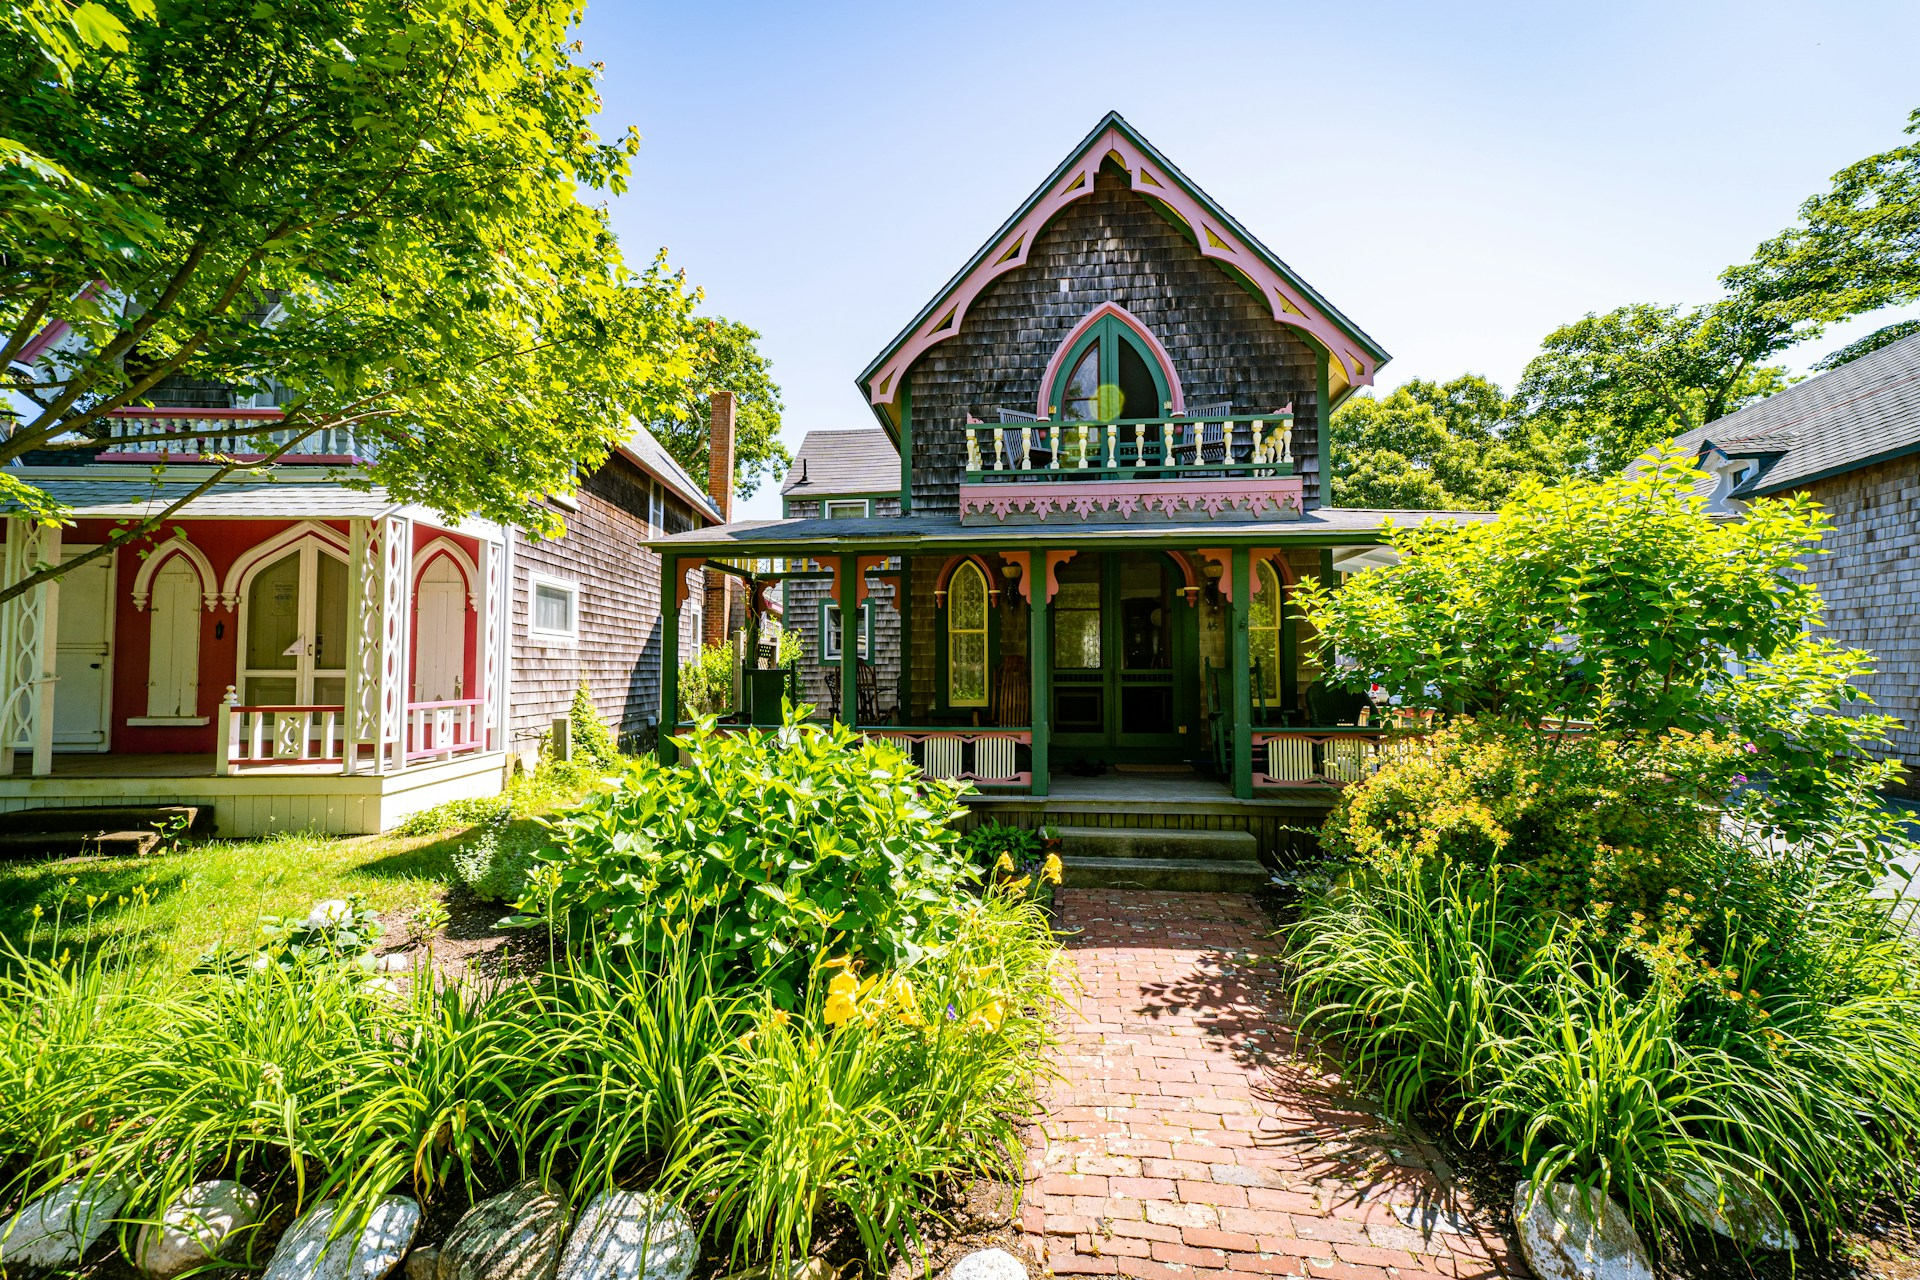
\includegraphics{images/mv-2.jpg}

}

\subcaption{Vineyard lighthouse}

\end{figure}%

\end{minipage}%

\end{figure}%

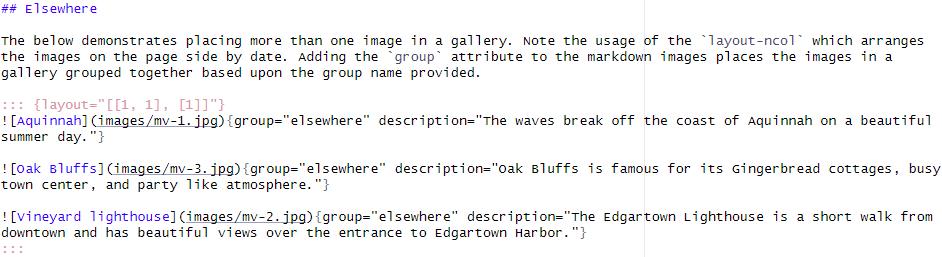
\includegraphics{images/_format_lightbox2.png}

\begin{figure}

\begin{minipage}{0.33\linewidth}

\begin{figure}[H]

{\centering 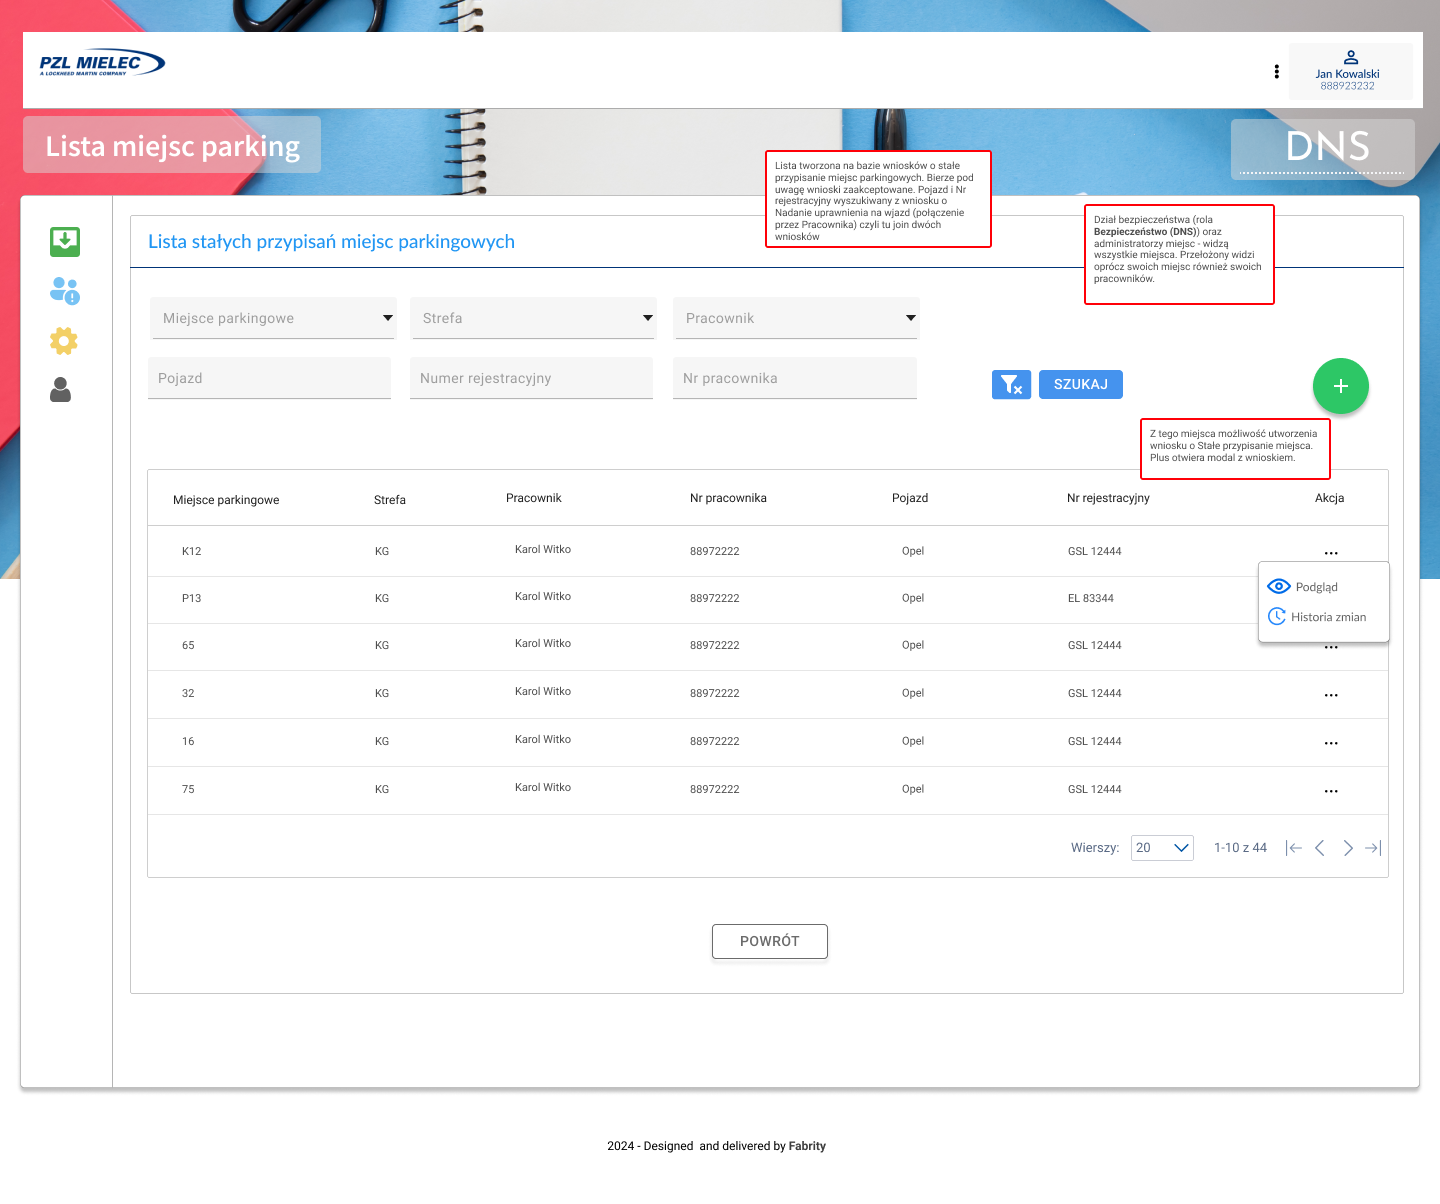
\includegraphics{images/wniosek1.png}

}

\subcaption{Makieta 1}

\end{figure}%

\end{minipage}%
%
\begin{minipage}{0.33\linewidth}

\begin{figure}[H]

{\centering 
\includegraphics{images/wniosek2.png}

}

\subcaption{Makieta 2}

\end{figure}%

\end{minipage}%
%
\begin{minipage}{0.33\linewidth}

\begin{figure}[H]

{\centering 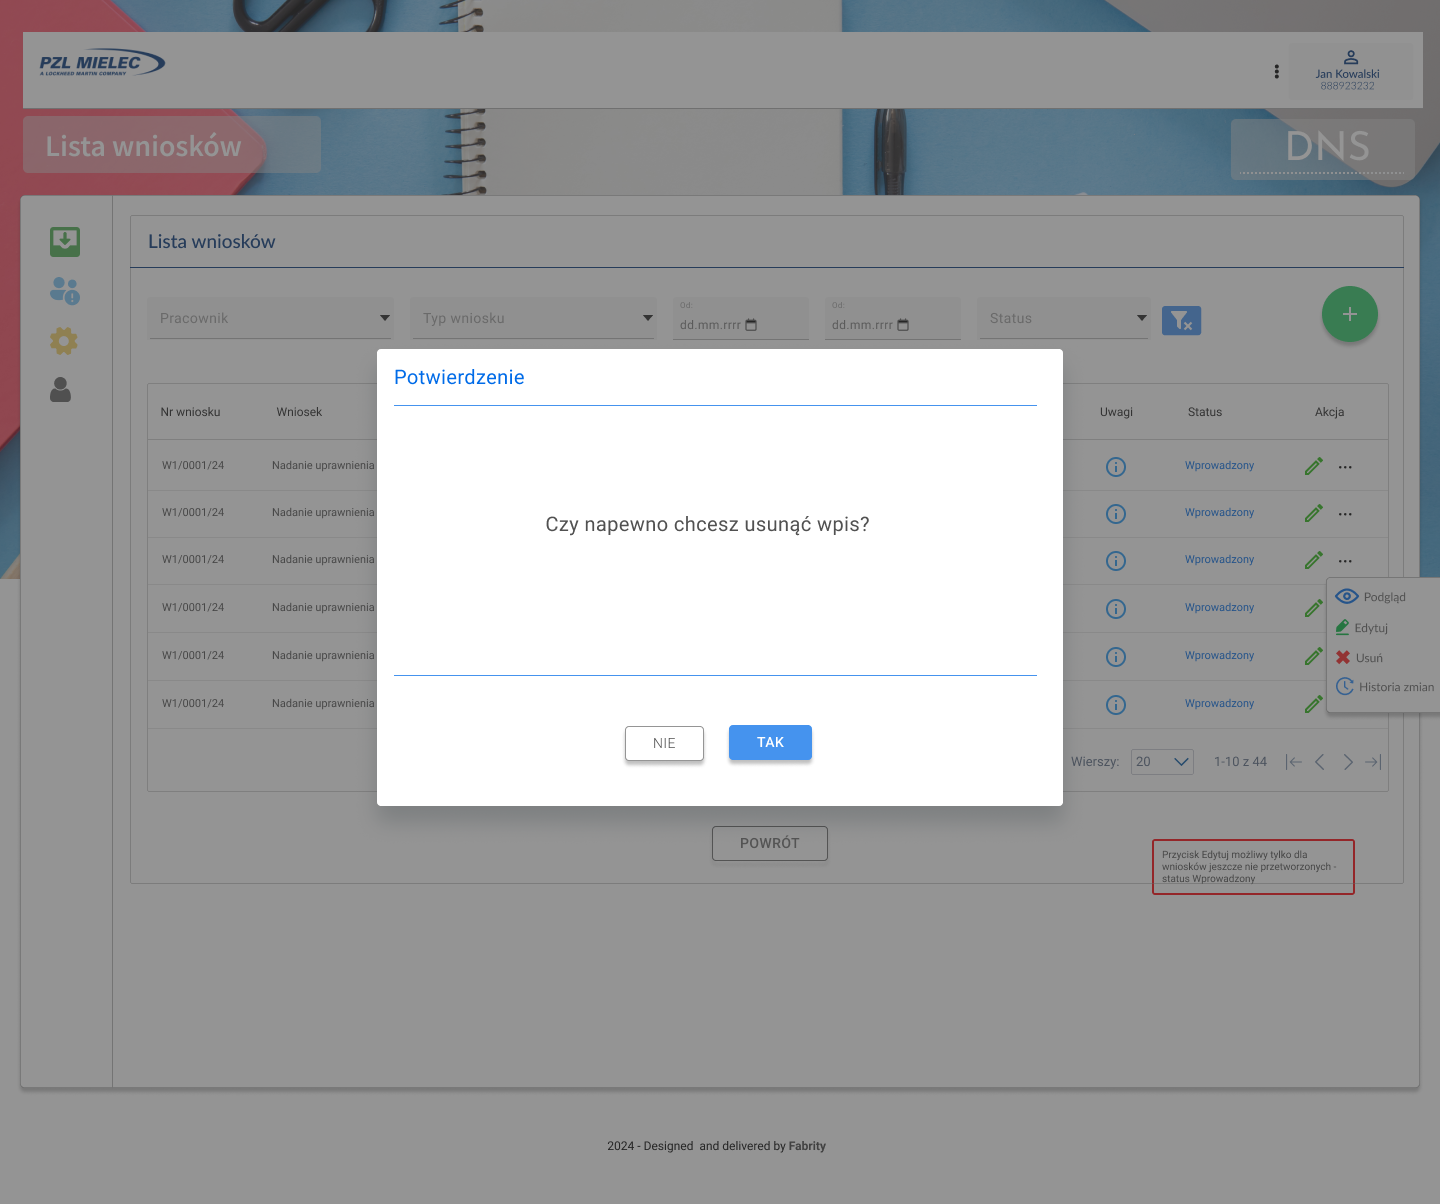
\includegraphics{images/wniosek3.png}

}

\subcaption{Makieta 3}

\end{figure}%

\end{minipage}%

\end{figure}%

\section{Asides}\label{asides}

\begin{itemize}
\tightlist
\item
  \textbf{Aside boczne}
\end{itemize}

{\marginnote{\begin{footnotesize}By ``right format'', we mean that the
data is tidy, and ready to be summarised and
graphed.\end{footnotesize}}}


\includegraphics{images/_format_aside.png}

\begin{center}\rule{0.5\linewidth}{0.5pt}\end{center}

\begin{itemize}
\tightlist
\item
  \textbf{Aside boczne callout}
\end{itemize}

\marginnote{\begin{footnotesize}

\begin{tcolorbox}[enhanced jigsaw, bottomrule=.15mm, titlerule=0mm, colbacktitle=quarto-callout-note-color!10!white, coltitle=black, rightrule=.15mm, opacitybacktitle=0.6, colframe=quarto-callout-note-color-frame, colback=white, breakable, arc=.35mm, toptitle=1mm, leftrule=.75mm, bottomtitle=1mm, title=\textcolor{quarto-callout-note-color}{\faInfo}\hspace{0.5em}{Uwaga}, toprule=.15mm, left=2mm, opacityback=0]

To jest przykładowy callout w sekcji bocznej.

\end{tcolorbox}

\end{footnotesize}}


\includegraphics{images/_format_aside2.png}

\begin{center}\rule{0.5\linewidth}{0.5pt}\end{center}

\section{Tabs}\label{tabs}

\begin{itemize}
\tightlist
\item
  \textbf{Tabsy}
\end{itemize}

\subsection{Plots}

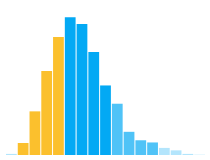
\includegraphics{images/altair-hist.png}

\subsection{Data}

If you want to allow users to toggle between multiple visualizations,
use a tabset (div with class .panel-tabset). Include a heading
(e.g.~\#\#) for each tab in the tabset.

For example, here are a plot and data each presented in their own tab.

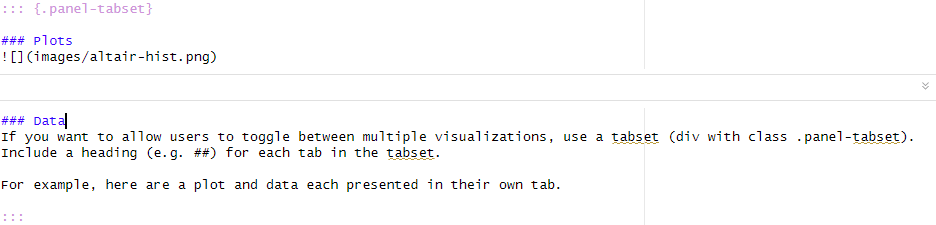
\includegraphics{images/_format_tabset.png}

\begin{center}\rule{0.5\linewidth}{0.5pt}\end{center}

\section{Glossary}\label{glossary}

Test słowa w słowniku, który jest tu zlikowanyt to We want to define the
term \hyperref[glossary-data-frame]{data frame} in the glossary


\includegraphics[width=5.28125in,height=\textheight]{images/_format_glossary.png}

a w samym słowniku glossary.qmd definiujesz pojęcie:


\includegraphics{images/_format_glossary2.png}

\bookmarksetup{startatroot}

\chapter*{References}\label{references}
\addcontentsline{toc}{chapter}{References}

\markboth{References}{References}

\phantomsection\label{refs}
\begin{CSLReferences}{1}{0}
\bibitem[\citeproctext]{ref-knuth84}
Knuth, Donald E. 1984. {``Literate Programming.''} \emph{Comput. J.} 27
(2): 97--111. \url{https://doi.org/10.1093/comjnl/27.2.97}.

\end{CSLReferences}

\cleardoublepage
\phantomsection
\addcontentsline{toc}{part}{Appendices}
\appendix

\chapter{Glossary}\label{sec-glossary}

\begin{description}
\item[\phantomsection\label{glossary-console}{Console}]
Coming soon.
\item[\phantomsection\label{glossary-data-frame}{Data frame}]
For our purposes, data frames are just R's term for data set or data
table. Data frames are made up of columns (variables) and rows
(observations). In R, all columns of a data frame must have the same
length.
\item[\phantomsection\label{glossary-functions}{Functions}]
Coming soon.
\end{description}

\begin{itemize}
\item
  \textbf{Arguments:} Arguments always go \emph{inside} the parentheses
  of a function and give the function the information it needs to give
  us the result we want.
\item
  \textbf{Pass:} In programming lingo, you \emph{pass} a value to a
  function argument. For example, in the funtion call
  \texttt{seq(from\ =\ 2,\ to\ =\ 100,\ by\ =\ 2)} we could say that we
  passed a value of 2 to the \texttt{from} argument, we passed a value
  of 100 to the \texttt{to} argument, and we passed a value of 2 to the
  \texttt{by} argument.
\item
  \textbf{Returns:} Instead of saying, ``the \texttt{seq()} function
  \emph{gives us} a sequence of numbers\ldots{}'' we could say, ``the
  \texttt{seq()} function \emph{returns} us a sequence of
  numbers\ldots{}'' In programming lingo, functions \emph{return} one or
  more results.
\end{itemize}

\begin{description}
\item[\phantomsection\label{glossary-global-environment}{Global
environment}]
Coming soon.
\item[\phantomsection\label{glossary-objects}{Objects}]
Coming soon.
\end{description}




\end{document}
